% =====================================================================
% APS - Laboratório de Projeto de Banco de Dados (UNIP São José dos Campos)
% Banco de dados de telemetria IoT para dados críticos
% Classe abnTeX2 (ABNT NBR 14724) + biblatex-abnt (NBR 6023 / NBR 10520)
% Compilar: latexmk -pdf main.tex   (ou pdflatex -> biber -> pdflatex x2)
% =====================================================================
\documentclass[
  12pt, oneside, a4paper,
  english, brazil,
  sumario=tradicional
]{abntex2}

% ---------------------------------------------------------------------
% Pacotes
% ---------------------------------------------------------------------
\usepackage[T1]{fontenc}
\usepackage[utf8]{inputenc}
\usepackage[scaled=0.95]{helvet}          % fonte sem serifa (padrão do grupo)
\renewcommand{\familydefault}{\sfdefault}
\renewcommand{\ttdefault}{txtt}        % monoespaçada mais encorpada (txfonts)
\usepackage{microtype}
\usepackage{csquotes}
\setlength{\emergencystretch}{3em}
\renewcommand{\topfraction}{0.92}\renewcommand{\bottomfraction}{0.8}\renewcommand{\textfraction}{0.06}\renewcommand{\floatpagefraction}{0.75}\setcounter{topnumber}{3}\setcounter{bottomnumber}{2}\setcounter{totalnumber}{4}
\usepackage{indentfirst}
\usepackage{graphicx}
\usepackage{xcolor}
\usepackage{booktabs}
\usepackage{tabularx}
\usepackage{multirow}
\usepackage{array}
\usepackage{siunitx}
\sisetup{output-decimal-marker={,}, group-separator={.}, group-minimum-digits=4}
\usepackage{tikz}
\usetikzlibrary{arrows.meta,shapes.geometric,shapes.symbols,calc,positioning}
\usepackage{pgf-umlcd}
\usepackage{pgfplots}
\pgfplotsset{compat=1.18}
\usepackage{listings}
\usepackage{enumitem}
\setlist{nosep, leftmargin=*, labelindent=\parindent}

% Referências e citações: ABNT NBR 6023 e NBR 10520
\usepackage[
  style=abnt,
  backend=biber,
  justify,
  extrayear,
  repeatfields,
  natbib=false,
  noslsn
]{biblatex}
% ---------------------------------------------------------------------
% Citações conforme ABNT NBR 10520:2023
% - sobrenome em maiúsculas e minúsculas também dentro dos parênteses:
%   (Sommerville, 2018), e não (SOMMERVILLE, 2018)
% - siglas de entidades continuam em maiúsculas: (CEMADEN, 2024)
% - referências seguem com o SOBRENOME em maiúsculas (NBR 6023:2025)
% O biblatex-abnt aplica a caixa alta nas citações pela macro
% \UpperOrSCCite; aqui ela passa a manter o nome como está.
% ---------------------------------------------------------------------
\makeatletter
\AtEndPreamble{\renewcommand*{\UpperOrSCCite}[1]{#1}}
\makeatother
% "et al." em itálico (NBR 10520:2023, 4 ou mais autores)
\DefineBibliographyStrings{brazil}{andothers = {\mkbibemph{et al\adddot}}}

% DOI como endereço completo (ABNT NBR 6023:2025)
\DeclareFieldFormat{doi}{DOI: \url{https://doi.org/#1}}

\addbibresource{referencias.bib}

\definecolor{azul}{HTML}{1F6FB2}
\definecolor{azulclaro}{HTML}{E3EEF8}
\definecolor{verde}{HTML}{2E8A57}
\definecolor{verdeclaro}{HTML}{E2F2E8}
\definecolor{tinta}{HTML}{15242F}
\definecolor{cinza}{HTML}{6D7F8C}
\definecolor{cinzaclaro}{HTML}{EEF2F4}


% ---------------------------------------------------------------------
% Quadros (texto) separados de tabelas (dados numéricos), como pede a ABNT
% ---------------------------------------------------------------------
\newcommand{\quadroname}{Quadro}
\newcommand{\listofquadrosname}{Lista de quadros}
\newfloat[chapter]{quadro}{loq}{\quadroname}
\newlistof{listofquadros}{loq}{\listofquadrosname}
\newlistentry{quadro}{loq}{0}
\setfloatadjustment{quadro}{\centering}
\counterwithout{quadro}{chapter}
\renewcommand{\cftquadroname}{\quadroname\space}
\renewcommand*{\cftquadroaftersnum}{\hfill--\hfill}

% numeração contínua de figuras e tabelas (NBR 14724)
\counterwithout{figure}{chapter}
\counterwithout{table}{chapter}

% colunas de quadros/tabelas
\newcolumntype{L}[1]{>{\raggedright\arraybackslash}p{#1}}
\newcolumntype{Y}{>{\raggedright\arraybackslash}X}
\renewcommand{\arraystretch}{1.25}

% código SQL curto
\renewcommand{\lstlistingname}{Código}
\lstset{
  basicstyle=\ttfamily\footnotesize, keywordstyle=\color{azul}\bfseries,
  commentstyle=\color{cinza}\itshape, stringstyle=\color{verde},
  frame=single, rulecolor=\color{cinza!50}, breaklines=true, columns=fullflexible,
  showstringspaces=false, language=SQL, morekeywords={RETURNING,ATTACH,DETACH,PARTITION,POLICY,EXECUTE,FUNCTION,TRIGGER},
  literate={á}{{\'a}}1 {ã}{{\~a}}1 {â}{{\^a}}1 {é}{{\'e}}1 {ê}{{\^e}}1 {í}{{\'i}}1 {ó}{{\'o}}1 {õ}{{\~o}}1 {ô}{{\^o}}1 {ú}{{\'u}}1 {ç}{{\c c}}1 {Ç}{{\c C}}1
}

% ---------------------------------------------------------------------
% Dados do trabalho
% ---------------------------------------------------------------------
\titulo{Banco de dados de telemetria IoT para dados críticos: plataforma de monitoramento meteorológico para a Defesa Civil de São José dos Campos}
\autor{%
  RA N062576 -- Gabriel Marques\\
  RA G8659C1 -- Gabriel Luiz Bastos Pereira\\
  RA N050FA1 -- Diego Ferraz\\
  RA N454830 -- Pedro Henrique de Souza Lemos\\
  RA G773470 -- Wellington Tomiyoshi Santos Koga}
\local{São José dos Campos}
\data{2026}
\orientador{Prof. Fernando Mauro}
\instituicao{%
  UNIP -- Universidade Paulista
  \par
  Curso de Engenharia da Computação}
\tipotrabalho{Atividade Prática Supervisionada}
\preambulo{Atividade Prática Supervisionada apresentada ao curso de Engenharia da Computação da Universidade Paulista -- UNIP, campus São José dos Campos, disciplina de Laboratório de Projeto de Banco de Dados (LPBD), como requisito parcial de avaliação.}

\makeatletter
\hypersetup{
  pdftitle={\@title}, pdfauthor={Grupo APS LPBD}, pdfsubject={\imprimirpreambulo},
  pdfcreator={LaTeX com abnTeX2}, pdfkeywords={banco de dados}{dados críticos}{PostgreSQL}{IoT}{auditoria},
  colorlinks=true, linkcolor=black, citecolor=black, filecolor=black, urlcolor=azul, bookmarksdepth=4
}
\makeatother

% espaço depois de \fonte e legenda das figuras
\setlength{\absparsep}{18pt}
\makeindex

\begin{document}
\selectlanguage{brazil}
\frenchspacing

% =====================================================================
% ELEMENTOS PRÉ-TEXTUAIS
% =====================================================================
\pretextual

% ---- Capa (identificação dos integrantes com RA na folha de rosto)
\renewcommand{\imprimircapa}{%
  \begin{capa}%
    \center
    {\ABNTEXchapterfont\large\MakeUppercase{UNIP -- Universidade Paulista}}
    \vspace*{0.6cm}

    {\large Curso de Engenharia da Computação}
    \vspace*{1.6cm}

    {\large Gabriel Marques\\Gabriel Luiz Bastos Pereira\\Diego Ferraz\\Pedro Henrique de Souza Lemos\\Wellington Tomiyoshi Santos Koga\par}
    \vfill
    \begin{center}
      \ABNTEXchapterfont\bfseries\Large\imprimirtitulo
    \end{center}
    \vspace*{0.8cm}

    {\large Atividade Prática Supervisionada}
    \vfill
    \large\imprimirlocal\par
    \large\imprimirdata
    \vspace*{1cm}
  \end{capa}}
\imprimircapa

% ---- Folha de rosto
\imprimirfolhaderosto

% ---- Resumo e abstract
% ---------------------------------------------------------------------
% Resumo (NBR 6028: parágrafo único, 150 a 500 palavras, voz ativa)
% ---------------------------------------------------------------------
\setlength{\absparsep}{18pt}
\begin{resumo}
Dados de monitoramento de chuva e vento usados pela Defesa Civil são dados críticos: um valor perdido, adulterado ou atrasado pode atrasar um alerta de deslizamento ou alagamento. Este trabalho apresenta o projeto e o protótipo de um banco de dados de telemetria IoT em PostgreSQL, aplicado a duas estações meteorológicas simuladas em São José dos Campos (SP), que medem temperatura e umidade do ar, chuva, direção e velocidade do vento e radiação solar a cada minuto e transmitem lotes a cada dez minutos. A partir de uma versão inicial focada em desempenho, o grupo levantou requisitos de dados críticos e implementou, no próprio banco, a validação de cada leitura com datas vindas somente do relógio do servidor, eventos imutáveis, papéis de mínimo privilégio, isolamento por cliente com \textit{Row Level Security}, senhas com bcrypt e bloqueio por tentativas, e uma trilha de auditoria somente de inclusão encadeada por hash SHA-256. Um servidor em Node.js e um painel em HTML, CSS e JavaScript puros completam o protótipo, com atualização em tempo real, backups diários verificados e uma fila de contingência que guarda os lotes quando o banco está fora do ar. Seis meses de operação (cerca de 529 mil leituras) foram simulados e os mecanismos foram testados: a adulteração proposital da auditoria foi detectada no registro exato, o PostgreSQL foi derrubado durante o envio de dados sem perda de leituras, e uma cópia de segurança foi restaurada com as mesmas contagens e a trilha de auditoria íntegra. As consultas mantiveram os ganhos das otimizações (até 200 vezes com view materializada), e as validações aumentaram em cerca de 30\,\% o tempo de envio de uma leitura por vez, com impacto desprezível em lotes de dez. Conclui-se que um banco relacional bem modelado pode concentrar as garantias de integridade, confidencialidade, rastreabilidade e disponibilidade exigidas por dados críticos, sem depender da boa conduta da aplicação.

\vspace{\onelineskip}
\noindent\textbf{Palavras-chave}: banco de dados; dados críticos; PostgreSQL; auditoria; IoT.
\end{resumo}

\begin{resumo}[Abstract]
\begin{otherlanguage*}{english}
Rain and wind monitoring data used by civil defense agencies are critical data: a lost, tampered or delayed value may delay a landslide or flood warning. This work presents the design and prototype of an IoT telemetry database in PostgreSQL, applied to two simulated weather stations in São José dos Campos, Brazil, which measure air temperature and humidity, rainfall, wind direction and speed, and solar radiation every minute and transmit batches every ten minutes. Starting from a performance-oriented first version, the group gathered critical-data requirements and implemented, inside the database, validation of every reading with timestamps taken only from the server clock, immutable events, least-privilege roles, per-customer isolation with Row Level Security, bcrypt passwords with lockout, and an append-only audit trail chained by SHA-256 hashes. A Node.js server and a plain HTML, CSS and JavaScript dashboard complete the prototype, with real-time updates, verified daily backups and a contingency queue that keeps batches while the database is down. Six months of operation (about 529 thousand readings) were simulated and the mechanisms were tested: deliberate tampering of the audit trail was detected at the exact record, PostgreSQL was shut down while data was being sent without losing readings, and a backup was restored with identical row counts and an intact audit trail. Queries kept the gains of the optimizations (up to 200 times with a materialized view), and validation increased single-reading inserts by about 30\,\%, with negligible impact on ten-reading batches.

\vspace{\onelineskip}
\noindent\textbf{Keywords}: database; critical data; PostgreSQL; audit trail; IoT.
\end{otherlanguage*}
\end{resumo}


% ---- Sumário
\pdfbookmark[0]{\contentsname}{toc}
\settocdepth{section}
\tableofcontents*
\cleardoublepage

% =====================================================================
% ELEMENTOS TEXTUAIS
% =====================================================================
\textual

% =====================================================================
\chapter{Introdução}\label{cap:introducao}
% =====================================================================

Desastres hidrometeorológicos, como inundações e deslizamentos, estão entre os eventos que mais causam mortes e prejuízos no Brasil. Em 2024, o Centro Nacional de Monitoramento e Alertas de Desastres Naturais ampliou para 1.133 a lista de municípios monitorados \parencite{cemaden2024}, e só nesses municípios foram registrados, em 2023, 815 eventos de inundação e 526 deslizamentos \parencite[p.~70]{nakano2024}. No Litoral Norte paulista, vizinho ao Vale do Paraíba, os pluviômetros registraram em fevereiro de 2023 663~mm de chuva em 24 horas em Bertioga \parencite{metsul2023}.

Cabe aos municípios manter a população informada sobre áreas de risco e eventos extremos \parencite{lei12608}, e para isso a Defesa Civil depende de dados que chegam continuamente de estações em campo. Esses dados são \textbf{críticos}: se uma leitura de chuva se perde, é alterada sem registro ou chega tarde, o alerta pode não acontecer. Por isso, além de rápido, o banco de dados que os recebe precisa garantir integridade, controle de acesso, rastreabilidade e continuidade.

\textbf{Problema.} Uma primeira versão do banco, feita pelo grupo, já recebia leituras em volume e gerava alarmes, mas não protegia o dado: todos os acessos usavam o superusuário, não havia registro de quem alterava regras, uma leitura com data inválida derrubava o lote inteiro e as partições mensais acabariam em dezembro de 2026, o que faria toda transmissão falhar a partir de janeiro.

\textbf{Objetivo.} Projetar e prototipar um banco de dados de telemetria IoT em PostgreSQL adequado a dados críticos, com servidor e painel web, e comprovar suas garantias com testes. Especificamente: apresentar os conceitos envolvidos; levantar requisitos e modelar o sistema; implementar no banco validação, auditoria, controle de acesso e continuidade; e medir o custo dessas garantias no desempenho.

\textbf{Escopo.} Foram implementados o banco de dados, um servidor em Node.js e um painel em HTML, CSS e JavaScript. O equipamento de campo e o meio de transmissão foram substituídos por um simulador que gera leituras realistas para duas estações da Defesa Civil de São José dos Campos, Centro e Zona Norte.

% =====================================================================
\chapter{Fundamentação teórica}\label{cap:fundamentacao}
% =====================================================================

\section{Banco de dados, SGBD e modelo relacional}

Um \textbf{banco de dados} é uma coleção de dados relacionados, organizada para um propósito; o \textbf{sistema gerenciador de banco de dados} (SGBD) é o software que permite defini-lo, manipulá-lo e compartilhá-lo entre aplicações e usuários \parencite{elmasri2018}. Em vez de cada programa tratar acesso concorrente, recuperação de falhas, integridade e autorização, o SGBD assume essas tarefas para todos \parencite{silberschatz2020}. Essa centralização é o ponto de partida deste trabalho: uma regra que vive só na aplicação pode ser contornada por outro programa; uma regra que vive no SGBD vale para todos.

O modelo relacional representa os dados como tabelas manipuladas por operações sobre conjuntos \parencite{codd1970}. Sobre ele, o SGBD garante restrições declaradas no esquema: \textbf{chave primária} (no projeto, estação mais data e hora impede gravar a mesma leitura duas vezes), \textbf{chave estrangeira} (um sensor só pertence a uma estação existente) e \textbf{\texttt{CHECK}} (o perfil do usuário só pode ser administrador, operador ou visualizador). A tabela de leituras usa o \textbf{formato largo}, uma coluna por grandeza, que reduz linhas e simplifica consultas quando as grandezas são fixas.

\section{Transações e durabilidade}

Uma \textbf{transação} é uma unidade de trabalho com as propriedades ACID: atomicidade (tudo ou nada), consistência (de um estado válido a outro), isolamento (transações concorrentes não se enxergam pela metade) e durabilidade (o que foi confirmado sobrevive a falhas) \parencite{harder1983}. A durabilidade vem do registro antecipado em log (\textit{write-ahead logging}, WAL): o SGBD grava a alteração no log antes de confirmá-la e, após uma queda, refaz o que foi confirmado \parencite{mohan1992}. No PostgreSQL, esse log também permite a recuperação para qualquer instante (PITR) \parencite{pgbackup}. No projeto, receber um lote é uma transação: leituras, eventos e alarmes entram juntos ou não entram.

\section{Programação no servidor e desempenho}

O PostgreSQL executa lógica dentro do banco em PL/pgSQL \parencite{pgdocs}: \textbf{funções} encapsulam operações (uma função \texttt{SECURITY DEFINER} roda com os privilégios de quem a criou, liberando uma operação sem liberar a tabela); \textbf{\textit{triggers}} rodam automaticamente a cada inclusão, alteração ou exclusão, sem que a aplicação possa evitá-los; e \textbf{\textit{event triggers}} reagem a comandos de estrutura como \texttt{ALTER} e \texttt{DROP}.

Para o desempenho com séries temporais \parencite{jensen2017,grzesik2020}, o projeto usa: \textbf{índice B-tree composto} (estação, data e hora), que no PostgreSQL 18 também serve a consultas só por período, graças ao \textit{skip scan} \parencite{pg18release}; \textbf{índice BRIN}, muito pequeno, para dados gravados em ordem de tempo; \textbf{particionamento mensal}, em que o banco lê só os meses consultados e move um mês inteiro para o arquivo sem copiar linhas; e \textbf{view materializada}, que guarda agregações prontas para os painéis \parencite{chirkova2012}.

\section{Dados críticos e segurança da informação}\label{sec:fund-criticos}

Neste trabalho, \textbf{dado crítico} é aquele cuja perda, alteração indevida, exposição ou indisponibilidade pode causar dano relevante a pessoas. A segurança da informação organiza sua proteção em \textbf{confidencialidade}, \textbf{integridade} e \textbf{disponibilidade} \parencite{iso27001}, com controles como gestão de acesso, registro de eventos e cópias de segurança \parencite{iso27002}; a LGPD exige medidas técnicas que protejam dados pessoais de acessos não autorizados \parencite{lgpd2018}. Os conceitos usados no protótipo são:

\begin{itemize}
  \item \textbf{mínimo privilégio}: cada programa e usuário opera só com os privilégios de que precisa \parencite{saltzer1975}. No banco, isso se faz com papéis distintos e com a segurança em nível de linha (\textit{Row Level Security}, RLS), que filtra quais linhas cada usuário vê \parencite{pgrls};
  \item \textbf{senhas com bcrypt}: função de hash propositalmente lenta e com \textit{salt}, que dificulta ataques de força bruta \parencite{provos1999};
  \item \textbf{auditoria à prova de adulteração}: cada registro guarda o hash do anterior, de modo que alterar ou apagar um registro quebra a corrente e se torna detectável \parencite{schneier1999,haber1991};
  \item \textbf{RPO e RTO}: quanto dado se aceita perder e em quanto tempo o serviço deve voltar após uma falha \parencite{nist80034};
  \item \textbf{segurança da aplicação web}: proteção contra controle de acesso quebrado e injeção de SQL e de scripts (XSS), as falhas mais comuns segundo a OWASP \parencite{owasp2021}.
\end{itemize}

% =====================================================================
\chapter{Plano de desenvolvimento, arquitetura e requisitos}\label{cap:arquitetura}
% =====================================================================

O problema foi organizado com o método 5W2H, já usado pelo grupo: o quê (receber e guardar leituras que geram alertas, com garantias de dado crítico), por quê (uma leitura perdida ou adulterada atrasa um alerta), onde (estações em campo, servidor da Defesa Civil e navegador dos operadores), quando (uma leitura por minuto e um lote a cada 10 minutos, sem parar), quem (dispositivos, operadores, órgãos de consulta e administrador), como (PostgreSQL com regras e segurança internas, servidor Node.js e painel web) e quanto (só software livre). Em seguida, a primeira versão do banco foi executada do zero e submetida a casos de borda; o \autoref{qua:diagnostico} resume os problemas encontrados, que orientaram as melhorias. Cada melhoria foi feita numa ramificação própria no GitHub e testada recriando o banco do zero.

\begin{quadro}[htb]
  \caption{Problemas encontrados na primeira versão}\label{qua:diagnostico}
  \footnotesize
  \begin{tabularx}{\textwidth}{|L{5.9cm}|Y|}
    \hline
    \textbf{Problema observado} & \textbf{Risco para dados críticos} \\ \hline
    Partições criadas só na carga, até dezembro de 2026 & Toda transmissão falharia a partir de janeiro de 2027 \\ \hline
    Uma leitura com data inválida derrubava o lote inteiro & Uma leitura ruim descartava as outras nove \\ \hline
    Leituras com data no futuro eram aceitas; data de recebimento informada pelo chamador & Dado com data falsa entrava no histórico \\ \hline
    Reenvio de lote já gravado gerava falha de sensor & O log registrava falhas que não aconteceram \\ \hline
    Todos os acessos com o superusuário \texttt{postgres} & Sem confidencialidade nem separação de funções \\ \hline
    Sem registro de quem alterou regras ou reconheceu eventos & Um limite de alarme podia ser elevado sem rastro \\ \hline
    Sem backup e recuperação & Uma falha de disco apagaria o histórico \\ \hline
  \end{tabularx}
  \fonte{Elaborado pelos autores (2026).}
\end{quadro}

\section{Arquitetura}

A arquitetura segue as camadas sensor, borda e nuvem de \textcite{grzesik2020}, com um servidor de aplicação entre o banco e os usuários (\autoref{fig:arquitetura}). Cada estação mede a cada minuto e envia um lote em JSON a cada dez minutos, identificado por uma chave própria. O servidor recebe os lotes, atende o painel, envia atualizações em tempo real e executa tarefas agendadas. O banco concentra as regras: valida cada leitura, gera eventos e alarmes, controla o acesso e registra a auditoria.

\begin{figure}[htb]
  \caption{Arquitetura do sistema}\label{fig:arquitetura}
  \centering
  \resizebox{0.92\textwidth}{!}{% Arquitetura: sensor -> borda -> servidor -> banco, com papéis de acesso
\begin{tikzpicture}[
  font=\footnotesize,
  caixa/.style={draw=azul, line width=0.7pt, rounded corners=3pt, fill=azulclaro, align=center, inner sep=4pt},
  sub/.style={draw=azul!60, rounded corners=2pt, fill=white, align=center, inner sep=2.5pt, font=\scriptsize, minimum width=2.45cm},
  disco/.style={cylinder, shape border rotate=90, aspect=0.22, draw=cinza, fill=cinzaclaro, align=center, font=\scriptsize, minimum width=1.9cm, minimum height=1.05cm},
  seta/.style={-{Stealth[length=2.2mm]}, line width=0.7pt, color=tinta},
  rot/.style={font=\scriptsize\itshape, color=tinta, align=center, fill=white, inner sep=1pt},
]
% --- campo
\node[caixa, minimum width=2.6cm, minimum height=1.3cm] (est1) at (0,1.1) {\textbf{Estação Centro}\\sensores + datalogger};
\node[caixa, minimum width=2.6cm, minimum height=1.3cm] (est2) at (0,-1.1) {\textbf{Estação Zona Norte}\\sensores + datalogger};
\node[font=\scriptsize\bfseries, color=cinza] at (0,2.35) {CAMPO (BORDA)};

% --- servidor
\node[draw=azul, line width=0.8pt, rounded corners=4pt, minimum width=3.4cm, minimum height=5.4cm, fill=azulclaro!40] (srv) at (4.6,0) {};
\node[font=\small\bfseries, anchor=north] at (srv.north) {Servidor Node.js};
\node[sub] (api) at (4.6,1.75) {API HTTP (JSON)\\\texttt{/api/ingest}};
\node[sub] (sse) at (4.6,0.75) {Tempo real (SSE)};
\node[sub] (age) at (4.6,-0.2) {Agendador};
\node[sub] (bkp) at (4.6,-1.15) {Backup (\texttt{pg\_dump})};
\node[sub] (cont) at (4.6,-2.1) {Fila de contingência};

% --- banco
\node[draw=verde, line width=0.8pt, rounded corners=4pt, minimum width=3.6cm, minimum height=5.4cm, fill=verdeclaro!50] (bd) at (9.3,0) {};
\node[font=\small\bfseries, anchor=north, align=center] at (bd.north) {PostgreSQL};
\node[sub, draw=verde!70] at (9.3,1.75) {Papéis + RLS};
\node[sub, draw=verde!70] at (9.3,0.8) {Validação e triggers};
\node[sub, draw=verde!70] at (9.3,-0.15) {Partições mensais};
\node[sub, draw=verde!70] at (9.3,-1.1) {Auditoria encadeada};
\node[sub, draw=verde!70] at (9.3,-2.05) {WAL (durabilidade)};

% --- usuários e discos
\node[caixa, minimum width=2.6cm, minimum height=1.1cm] (nav) at (4.6,-4.1) {\textbf{Navegador}\\painel HTML/CSS/JS};
\node[disco] (dbak) at (0.6,-3.0) {cópias\\.dump};
\node[disco] (dfila) at (0.6,-4.45) {fila em\\disco};

% --- ligações
\coordinate (ent) at (2.35,1.75);
\draw[line width=0.7pt, color=tinta] (est1.east) -- (ent);
\draw[line width=0.7pt, color=tinta] (est2.east) -- (ent);
\draw[seta] (ent) -- (api.west);
\node[rot, align=center] at (2.05,0.0) {lote JSON\\a cada 10 min\\+ chave da\\estação};
\draw[seta, <->] (srv.east |- 0,1.2) -- node[rot, above]{token da\\sessão} (bd.west |- 0,1.2);
\draw[seta] (bd.west |- 0,-0.55) -- node[rot, below]{NOTIFY} (srv.east |- 0,-0.55);
\draw[seta, <->] (nav.north) -- node[rot, right]{HTTPS\,/\,SSE} (srv.south);
\draw[seta, dashed] (bkp.west) -- ++(-0.95,0) |- (dbak.east);
\draw[seta, dashed] (cont.west) -- ++(-0.75,0) |- (dfila.east);
\end{tikzpicture}
}
  \fonte{Elaborado pelos autores (2026), adaptado de \textcite{grzesik2020}.}
\end{figure}

A decisão central é que o banco \textbf{não confia na aplicação}: o servidor se conecta com papéis de privilégio mínimo e repassa apenas o \textit{token} da sessão do usuário; é o banco que o valida e descobre quem é o usuário, seu perfil e as estações que pode ver. Mesmo com o servidor web comprometido, um invasor não se passa por outro usuário sem um \textit{token} válido.

\section{Metodologia de simulação e testes}

Um simulador gera leituras realistas (ciclo dia e noite, sazonalidade, tardes chuvosas e um dia de temporal), com cerca de 2\,\% de lotes atrasados e 0,5\,\% de leituras com o código de erro $-9999$. A carga cobre seis meses; depois, o servidor continua transmitindo em tempo real. Os testes foram de segurança (tentar burlar cada regra, inclusive como superusuário), de continuidade (derrubar o banco, fazer e restaurar backups) e de desempenho, com a metodologia de \textcite{grzesik2020}: escrita de 1.000 pontos, um por envio e em lotes de dez, e consultas de agregação repetidas 500 vezes em quatro cenários, antes e depois das melhorias, no mesmo ambiente.

\section{Requisitos funcionais e não funcionais}\label{cap:requisitos}

Requisitos funcionais descrevem os serviços do sistema; não funcionais restringem o sistema como um todo, como segurança e desempenho \parencite{sommerville2018}. Com dados críticos, os não funcionais pesam tanto quanto os funcionais: um sistema que gera o alarme certo mas perde dados numa queda não serve ao seu propósito \parencite{pressman2021}. Os quadros a seguir listam os requisitos levantados.

\begin{quadro}[htb]
  \caption{Requisitos funcionais}\label{qua:rf}
  \footnotesize
  \begin{tabularx}{\textwidth}{|c|Y|}
    \hline
    \textbf{ID} & \textbf{Descrição} \\ \hline
    RF01 & Receber lotes de leituras em JSON, identificando a estação por chave própria. \\ \hline
    RF02 & Validar cada leitura (data ausente, inválida, futura, antiga ou de mês arquivado) sem descartar o restante do lote. \\ \hline
    RF03 & Usar somente o relógio do servidor em toda data de registro; nenhum usuário digita data. \\ \hline
    RF04 & Detectar falhas de sensor e de transmissão, calcular a chuva do dia e gerar alarmes pelas regras configuradas. \\ \hline
    RF05 & Exibir painel em tempo real, gráficos, chuva por dia, histórico e exportação em CSV. \\ \hline
    RF06 & Permitir ao operador reconhecer eventos, registrando automaticamente quem e quando. \\ \hline
    RF07 & Permitir ajustar regras de alarme e faixas dos sensores (operador) e parâmetros do banco (administrador). \\ \hline
    RF08 & Gerenciar usuários com perfis, troca de senha no primeiro acesso e desbloqueio. \\ \hline
    RF09 & Auditar alterações, logins, exportações, backups e mudanças de estrutura, com antes e depois. \\ \hline
    RF10 & Verificar a integridade da auditoria e apontar o primeiro registro adulterado. \\ \hline
    RF11 & Fazer backup diário e sob demanda, verificar cada cópia e permitir a restauração. \\ \hline
    RF12 & Arquivar meses antigos e criar com antecedência as partições dos meses seguintes. \\ \hline
  \end{tabularx}
  \fonte{Elaborado pelos autores (2026).}
\end{quadro}

\begin{quadro}[htb]
  \caption{Requisitos não funcionais}\label{qua:rnf}
  \footnotesize
  \begin{tabularx}{\textwidth}{|c|L{2.6cm}|Y|}
    \hline
    \textbf{ID} & \textbf{Categoria} & \textbf{Descrição} \\ \hline
    RNF01 & Integridade & Regras implementadas no banco, que nenhuma aplicação contorna; eventos imutáveis. \\ \hline
    RNF02 & Confidencialidade & Papéis de mínimo privilégio, isolamento por cliente, senhas com bcrypt, sessões guardadas só como hash. \\ \hline
    RNF03 & Rastreabilidade & Auditoria somente de inclusão, encadeada por hash, que torne detectável qualquer alteração. \\ \hline
    RNF04 & Disponibilidade & Nenhuma leitura perdida com o banco fora do ar; perda máxima de 24 h com backup diário. \\ \hline
    RNF05 & Desempenho & Painel atualizado segundos após o lote; validações sem impacto relevante no envio em lote. \\ \hline
    RNF06 & Segurança web e portabilidade & Consultas parametrizadas, proteção contra CSRF e XSS; Windows e Linux com software livre. \\ \hline
  \end{tabularx}
  \fonte{Elaborado pelos autores (2026).}
\end{quadro}

% =====================================================================
\chapter{Modelagem do software}\label{cap:modelagem}
% =====================================================================

A modelagem usou a UML para casos de uso e classes \parencite{booch2006} e um diagrama entidade-relacionamento para o banco. Os atores são o \textbf{dispositivo} (datalogger que envia os lotes), o \textbf{visualizador} (consulta e exporta), o \textbf{operador} (também reconhece eventos e ajusta alarmes), o \textbf{administrador} (também gerencia usuários, auditoria, backups e parâmetros) e o \textbf{agendador} do servidor. A \autoref{fig:casos-uso} mostra os casos de uso; a herança entre atores representa os perfis cumulativos, e os «include» mostram que todo lote é validado e toda alteração é auditada.

\begin{figure}[htb]
  \caption{Diagrama de casos de uso}\label{fig:casos-uso}
  \centering
  \resizebox{0.74\textwidth}{!}{% Diagrama de casos de uso (UML)
\begin{tikzpicture}[
  font=\scriptsize,
  uc/.style={ellipse, draw=azul, fill=azulclaro, line width=0.6pt, minimum width=3.7cm, minimum height=0.8cm, align=center, inner sep=1pt},
  inc/.style={ellipse, draw=azul, dashed, fill=white, line width=0.6pt, minimum width=3.0cm, minimum height=0.72cm, align=center, inner sep=1pt},
  assoc/.style={line width=0.5pt, color=tinta},
  heranca/.style={-{Triangle[open, length=2.4mm, width=2.4mm]}, line width=0.5pt, color=tinta},
  inclui/.style={-{Stealth[length=1.8mm]}, dashed, line width=0.5pt, color=cinza},
]
\newcommand{\ator}[3]{%
  \begin{scope}[shift={#2}, line width=0.6pt, color=tinta]
    \draw (0,0.42) circle (0.13);
    \draw (0,0.29) -- (0,-0.08);
    \draw (-0.22,0.16) -- (0.22,0.16);
    \draw (0,-0.08) -- (-0.18,-0.38);
    \draw (0,-0.08) -- (0.18,-0.38);
    \node[font=\scriptsize\bfseries, align=center, below] at (0,-0.4) {#3};
    \coordinate (#1) at (0.25,0.1);
    \coordinate (#1-topo) at (0,0.6);
    \coordinate (#1-base) at (0,-0.95);
  \end{scope}}

\draw[rounded corners=6pt, draw=azul, line width=0.8pt] (-2.3,-5.15) rectangle (5.6,4.3);
\node[font=\scriptsize\bfseries, color=azul] at (1.65,4.02) {Sistema de monitoramento (banco + servidor + painel)};

\node[uc] (u1) at (0,3.3) {UC01 Enviar lote\\de leituras};
\node[uc] (u2) at (0,2.3) {UC02 Acompanhar painel\\em tempo real};
\node[uc] (u3) at (0,1.3) {UC03 Consultar gráficos,\\histórico e exportar};
\node[uc] (u4) at (0,0.3) {UC04 Reconhecer\\eventos};
\node[uc] (u5) at (0,-0.7) {UC05 Ajustar regras\\de alarme e sensores};
\node[uc] (u6) at (0,-1.7) {UC06 Gerenciar\\usuários};
\node[uc] (u7) at (0,-2.7) {UC07 Auditar e verificar\\integridade};
\node[uc] (u8) at (0,-3.7) {UC08 Fazer e verificar\\backup};
\node[uc] (u9) at (0,-4.6) {UC09 Arquivar dados\\e criar partições};

\node[inc] (i1) at (3.85,3.55) {Validar leituras\\e datas};
\node[inc] (i2) at (3.85,2.55) {Gerar eventos\\e alarmes};
\node[inc] (i3) at (3.85,-0.7) {Registrar na\\auditoria};

\ator{disp}{(-4.3,3.2)}{Dispositivo\\(datalogger)}
\ator{vis}{(-4.3,1.55)}{Visualizador}
\ator{ope}{(-4.3,-0.45)}{Operador}
\ator{adm}{(-4.3,-2.5)}{Administrador}
\ator{age}{(-4.3,-4.35)}{Agendador\\(servidor)}

\draw[assoc] (disp) -- (u1.west);
\draw[assoc] (vis) -- (u2.west);
\draw[assoc] (vis) -- (u3.west);
\draw[assoc] (ope) -- (u4.west);
\draw[assoc] (ope) -- (u5.west);
\draw[assoc] (adm) -- (u6.west);
\draw[assoc] (adm) -- (u7.west);
\draw[assoc] (adm) -- (u8.west);
\draw[assoc] (age) -- (u8.west);
\draw[assoc] (age) -- (u9.west);

\draw[heranca] (ope-topo) -- (vis-base);
\draw[heranca] (adm-topo) -- (ope-base);

\draw[inclui] (u1.east) -- node[above, font=\tiny, sloped]{«include»} (i1.west);
\draw[inclui] (u1.east) -- node[below, font=\tiny, sloped]{«include»} (i2.west);
\draw[inclui] (u4.east) -- node[above, font=\tiny, sloped]{«include»} (i3.west);
\draw[inclui] (u5.east) -- node[above, font=\tiny]{«include»} (i3.west);
\draw[inclui] (u6.east) -- node[below, font=\tiny, sloped]{«include»} (i3.west);
\end{tikzpicture}
}
  \fonte{Elaborado pelos autores (2026).}
\end{figure}

\newcommand{\linhauc}[2]{\textbf{#1} & #2 \\ \hline}

\begin{quadro}[htb]
  \caption{Caso de uso UC01 -- Enviar lote de leituras}\label{qua:uc01}
  \footnotesize
  \begin{tabularx}{\textwidth}{|L{2.8cm}|Y|}
    \hline
    \linhauc{Ator / pré-condição}{Dispositivo; estação ativa com chave de API cadastrada.}
    \textbf{Fluxo básico} & 1. O dispositivo envia o lote para \texttt{/api/ingest} com a chave no cabeçalho. 2. O banco identifica a estação pelo hash da chave e registra falha de transmissão se o lote atrasou. 3. Classifica cada leitura e separa as rejeitadas. 4. Grava as válidas e novas; os \textit{triggers} descartam valores fora da faixa, calculam a chuva acumulada e geram alarmes. 5. Registra a transmissão e avisa os painéis em tempo real. \\ \hline
    \textbf{Alternativos e exceções} & Leituras repetidas são ignoradas sem gerar eventos. Leituras inválidas geram um evento \texttt{LEITURA\_REJEITADA} por motivo, e o resto do lote é gravado. Chave inválida: envio recusado e auditado. Banco fora do ar: o lote vai para a fila de contingência. \\ \hline
    \linhauc{Regra}{A data de recebimento é sempre o relógio do servidor.}
  \end{tabularx}
  \fonte{Elaborado pelos autores (2026).}
\end{quadro}

\begin{quadro}[htb]
  \caption{Caso de uso UC07 -- Auditar e verificar integridade}\label{qua:uc07}
  \footnotesize
  \begin{tabularx}{\textwidth}{|L{2.8cm}|Y|}
    \hline
    \linhauc{Ator / pré-condição}{Administrador autenticado.}
    \textbf{Fluxo básico} & 1. O administrador abre a auditoria; a verificação roda sozinha. 2. O banco percorre a trilha em ordem, recalcula o SHA-256 de cada registro com o hash do anterior e compara com o gravado. 3. O administrador filtra por ação, objeto, usuário e período e abre o antes e depois de cada alteração. \\ \hline
    \linhauc{Alternativo}{Registro alterado ou removido: a tela mostra o número do primeiro registro com problema.}
    \linhauc{Regra}{A trilha é somente de inclusão; desligar essa proteção é um comando de estrutura e também é auditado.}
  \end{tabularx}
  \fonte{Elaborado pelos autores (2026).}
\end{quadro}

O diagrama de classes (\autoref{fig:classes}) representa o domínio. Suas operações estão no próprio banco, como funções e \textit{triggers} em PL/pgSQL: \texttt{receberLote} é \texttt{fn\_receber\_lote}, \texttt{reconhecer} é \texttt{fn\_reconhecer\_eventos} e \texttt{verificarIntegridade} é \texttt{fn\_verificar\_auditoria}.

\begin{figure}[htb]
  \caption{Diagrama de classes do domínio}\label{fig:classes}
  \centering
  \resizebox{0.84\textwidth}{!}{% Diagrama de classes do domínio (pgf-umlcd)
\begin{tikzpicture}[font=\scriptsize]
\begin{class}[text width=3.3cm]{Cliente}{0,0}
  \attribute{nome : texto}
  \attribute{cidade : texto}
  \attribute{uf : texto}
\end{class}

\begin{class}[text width=4.3cm]{Dispositivo}{5.2,0}
  \attribute{nome : texto}
  \attribute{status : Status}
  \attribute{ultimaComunicacao : data/hora}
  \attribute{intervaloTransmissao : int}
  \operation{+ receberLote(leituras) : int}
  \operation{+ verificarComunicacao()}
\end{class}

\begin{class}[text width=3.6cm]{Usuario}{0,-4.0}
  \attribute{login : texto}
  \attribute{senhaHash : bcrypt}
  \attribute{perfil : Perfil}
  \attribute{bloqueadoAte : data/hora}
  \operation{+ login(senha) : Sessao}
  \operation{+ alterarSenha(atual, nova)}
\end{class}

\begin{class}[text width=3.5cm]{Sessao}{0,-8.1}
  \attribute{tokenHash : SHA-256}
  \attribute{expiraEm : data/hora}
  \operation{+ validar() : Usuario}
\end{class}

\begin{class}[text width=3.6cm]{Sensor}{10.6,1.0}
  \attribute{parametro : texto}
  \attribute{limiteMin, limiteMax : num}
  \operation{+ valida(valor) : bool}
\end{class}

\begin{class}[text width=3.6cm]{RegraAlarme}{10.6,-2.3}
  \attribute{parametro : texto}
  \attribute{condicao : ACIMA/ABAIXO}
  \attribute{limite : num}
  \attribute{nivel : Nivel}
  \operation{+ violada(valor) : bool}
\end{class}

\begin{class}[text width=3.9cm]{Leitura}{5.2,-4.0}
  \attribute{dataHora : data/hora}
  \attribute{temperatura, umidade : num}
  \attribute{chuva, chuvaAcumulada : num}
  \attribute{vento, direcao, radiacao : num}
  \attribute{recebidoEm : data/hora}
\end{class}

\begin{class}[text width=3.6cm]{Evento}{5.2,-8.0}
  \attribute{dataHora : data/hora}
  \attribute{tipo : TipoEvento}
  \attribute{mensagem : texto}
  \attribute{reconhecidoEm : data/hora}
  \operation{+ reconhecer()}
\end{class}

\begin{class}[text width=4.4cm]{Auditoria}{10.6,-7.0}
  \attribute{dataHora, login, ip}
  \attribute{acao, antes, depois}
  \attribute{hashAnterior, hash}
  \operation{+ verificarIntegridade() : bool}
\end{class}

\association{Cliente}{}{1}{Dispositivo}{}{0..*}
\association{Cliente}{}{0..1}{Usuario}{}{0..*}
\composition{Usuario}{}{1}{Sessao}{0..*}
\composition{Dispositivo}{}{1}{Sensor}{1..*}
\composition{Dispositivo}{}{1}{RegraAlarme}{0..*}
\composition{Dispositivo}{}{1}{Leitura}{0..*}
\association{RegraAlarme}{gera}{0..1}{Evento}{}{0..*}
\association{Leitura}{origina}{1}{Evento}{}{0..*}
\association{Usuario}{reconhece}{0..1}{Evento}{}{0..*}
\end{tikzpicture}
}
  \fonte{Elaborado pelos autores (2026).}
\end{figure}

\section{Modelo de dados}

O modelo físico tem 14 tabelas (\autoref{fig:der}), num diagrama gerado do catálogo do banco para corresponder exatamente ao implementado. A tabela \texttt{leitura} tem uma linha por estação por minuto, chave primária (\texttt{id\_dispositivo}, \texttt{data\_hora}) e partições mensais; os meses antigos são movidos inteiros para \texttt{leitura\_arquivo}, com índice BRIN, e resumidos em \texttt{leitura\_diaria}. Os eventos ficam numa tabela única, no formato de log, com cinco tipos: transmissão OK, falha de transmissão, falha de sensor, alarme e leitura rejeitada. As regras de alarme cadastradas são chuva acumulada acima de 50~mm (crítico), vento acima de 17~m/s, temperatura acima de 35~°C e umidade abaixo de 20\,\% (alerta).

\begin{figure}[p]
  \caption{Modelo de dados (diagrama entidade-relacionamento)}\label{fig:der}
  \centering
  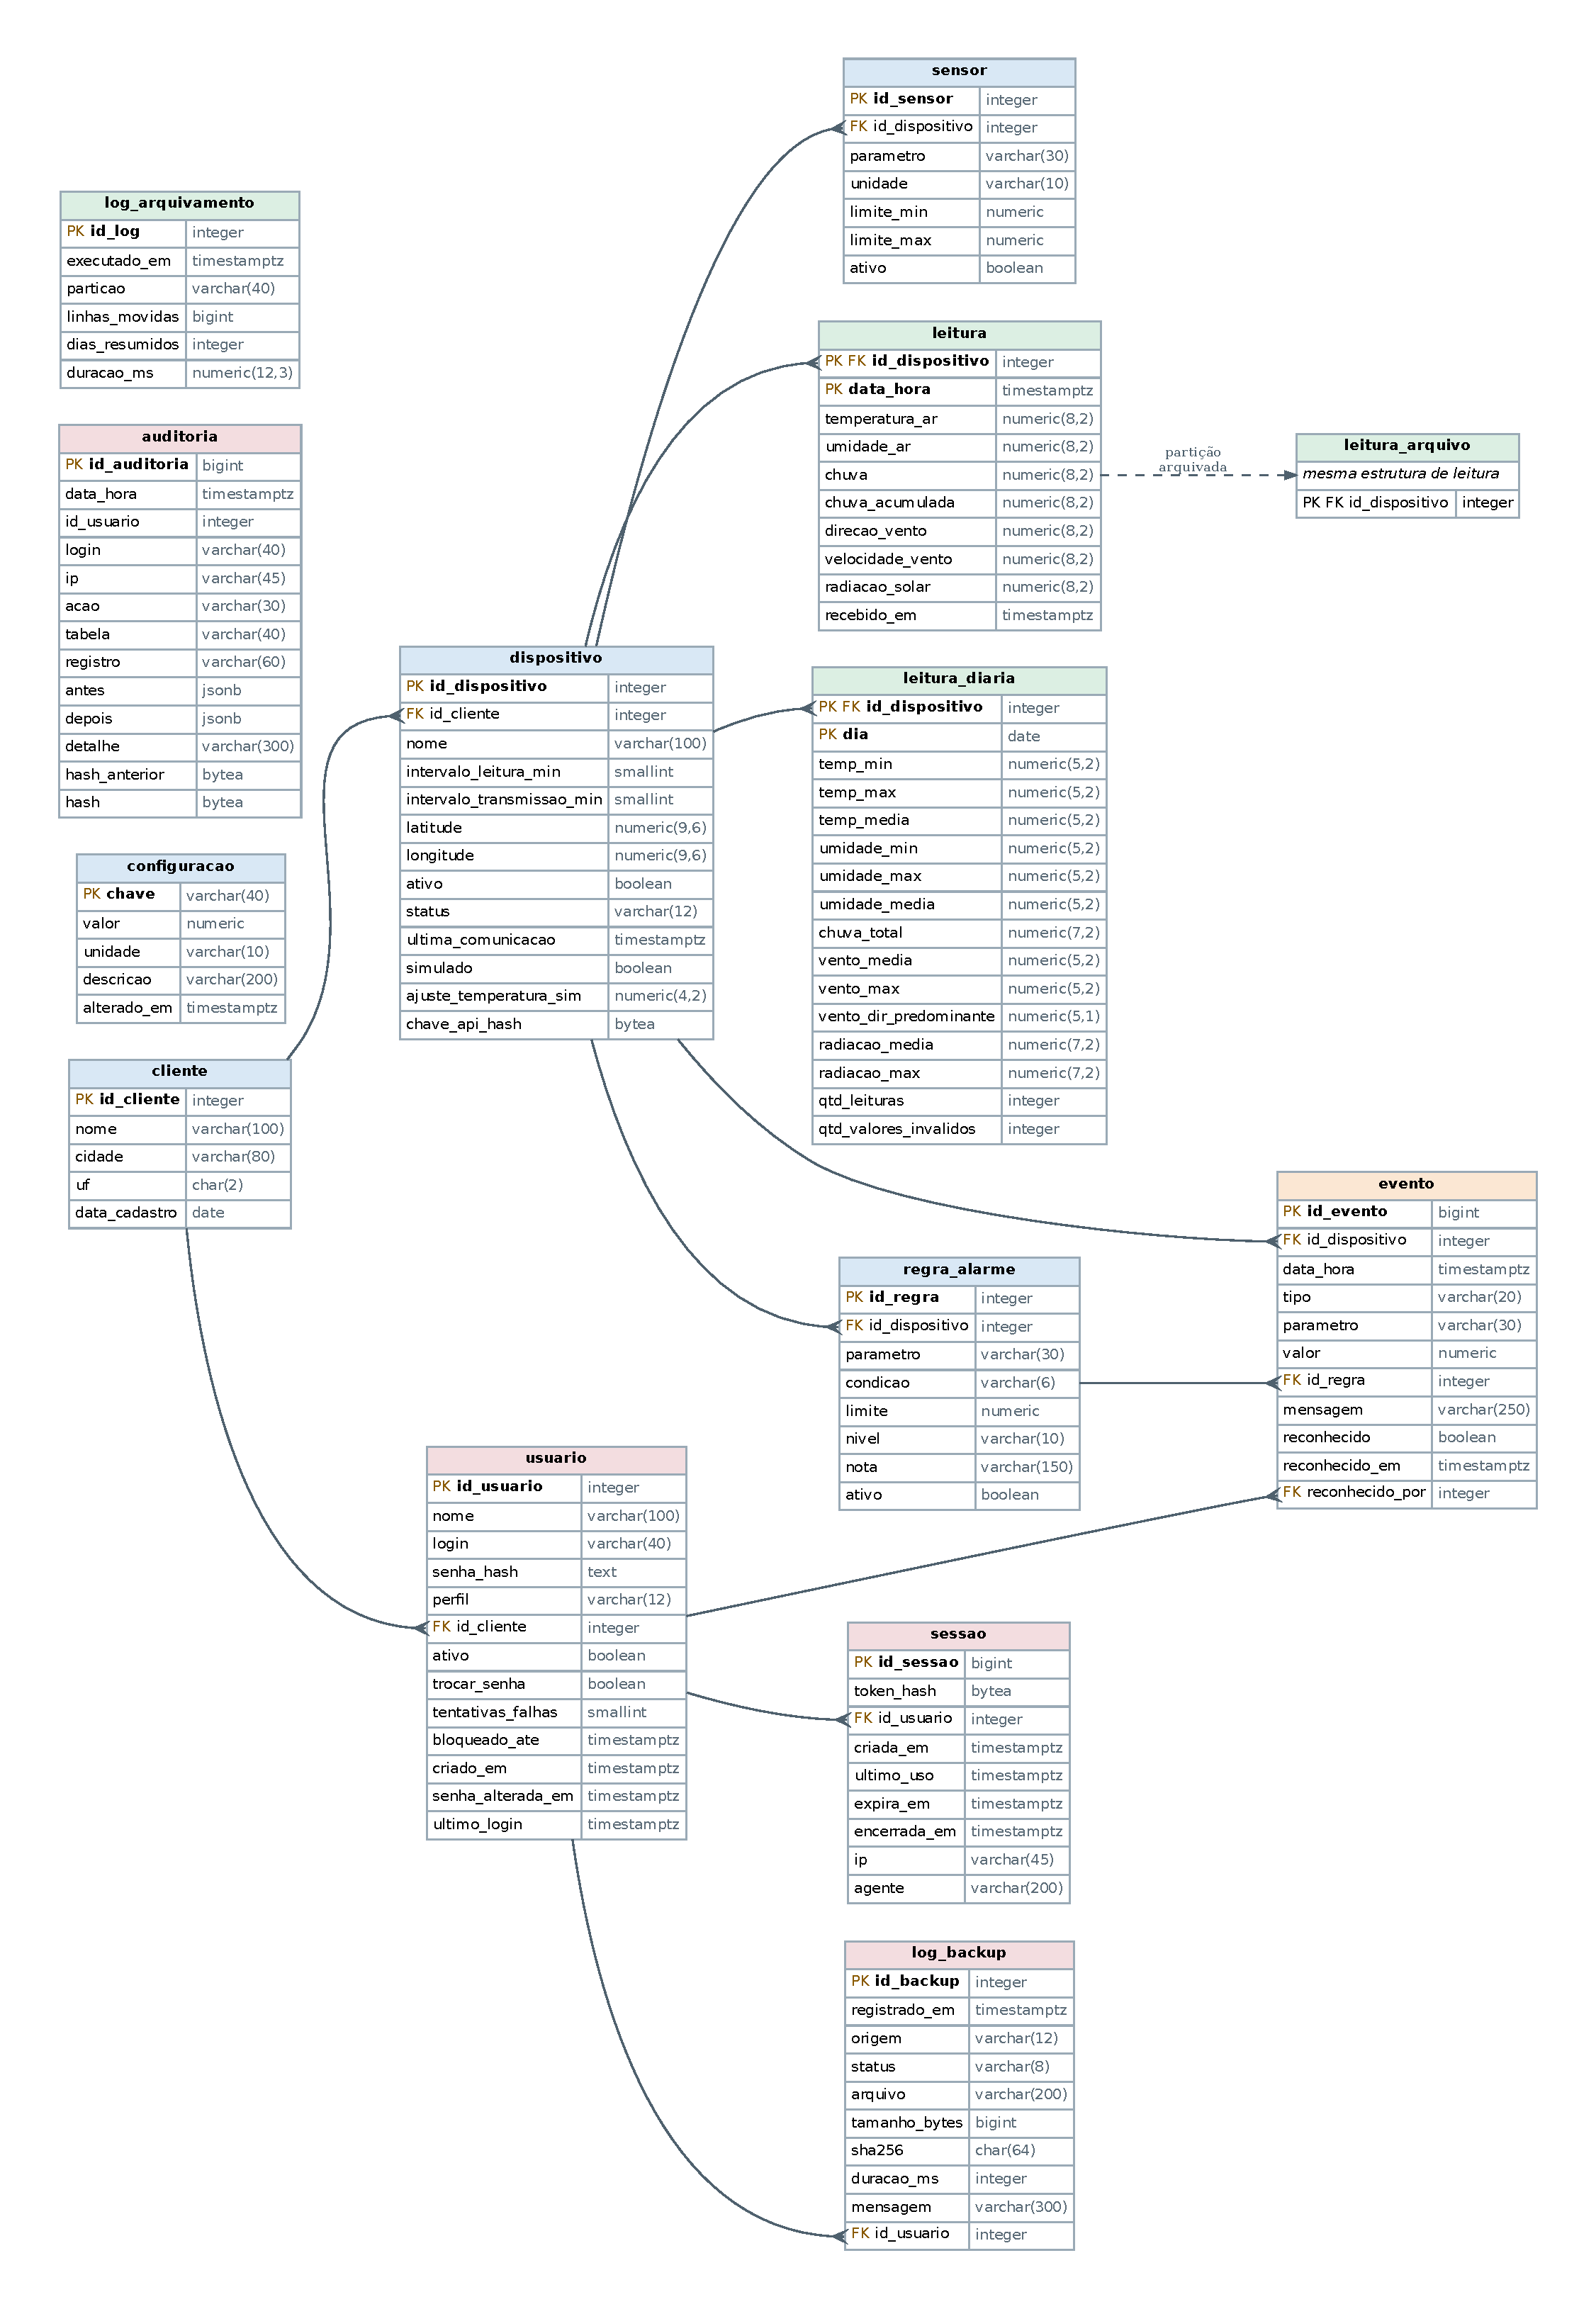
\includegraphics[height=0.84\textheight,width=\textwidth,keepaspectratio]{figuras/der.pdf}
  \fonte{Elaborado pelos autores (2026), gerado do catálogo do PostgreSQL com Graphviz.}
\end{figure}

\section{Regras implementadas no banco}

Todo dado entra por \texttt{fn\_receber\_lote}, que não tem parâmetro de data: o recebimento é sempre \texttt{now()}. Numa única instrução SQL, a função lê o JSON (valores mal formatados viram nulo, sem abortar o lote), classifica cada leitura (data no futuro além de 2~min, mais antiga que 7 dias ou de mês sem partição ativa são rejeitadas), grava um evento por motivo de rejeição e insere só as leituras válidas e novas, o que corrigiu as falhas de sensor ``fantasmas'' da primeira versão. Como defesa adicional, o \textit{trigger} da tabela recusa data no futuro mesmo em inclusões diretas.

Na auditoria, um \textit{trigger} define a data com o relógio do servidor, identifica o usuário pela sessão e calcula o SHA-256 do registro concatenado ao hash do anterior, sob um bloqueio que garante a ordem da corrente. Diariamente, o banco arquiva os meses antigos (\texttt{DETACH} e \texttt{ATTACH PARTITION}) e cria as partições dos dois meses seguintes.

% =====================================================================
\chapter{Protótipo}\label{cap:prototipo}
% =====================================================================

O protótipo é funcional: os scripts criam o banco do zero, o simulador gera seis meses de histórico e continua transmitindo em tempo real, e o painel opera sobre esses dados com usuários reais do banco. O código e as instruções de execução estão no repositório do grupo no GitHub (\url{https://github.com/Chulalafe3/APS_Banco_de_dados}).

% ---------------------------------------------------------------------
\section{Ferramentas utilizadas}
% ---------------------------------------------------------------------

\begin{quadro}[htbp]
  \caption{Ferramentas utilizadas}\label{qua:ferramentas}
  \footnotesize
  \begin{tabularx}{\textwidth}{|L{4.0cm}|Y|}
    \hline
    \textbf{Ferramenta} & \textbf{Uso no projeto} \\ \hline
    PostgreSQL (versões 16 a 18) & SGBD: armazenamento, regras, segurança, auditoria e recuperação \\ \hline
    PL/pgSQL & Funções, procedimentos, \textit{triggers} e \textit{event triggers} \\ \hline
    pgcrypto & bcrypt das senhas, SHA-256 da auditoria e das sessões, geração de \textit{tokens} \\ \hline
    pgAdmin 4 (PSQL Tool) & Execução dos scripts e consultas \\ \hline
    Node.js com o pacote \texttt{pg} & Servidor HTTP sem \textit{framework}: API, tempo real, agendador, backup e contingência \parencite{nodejs} \\ \hline
    HTML, CSS e JavaScript puros & Painel web com onze telas, gráficos em SVG próprios, sem bibliotecas externas \\ \hline
    Server-Sent Events & Envio das atualizações do servidor ao navegador em tempo real \parencite{mdnsse} \\ \hline
    \texttt{pg\_dump} e \texttt{pg\_restore} & Cópias de segurança, verificação e restauração \\ \hline
    Git e GitHub & Versionamento, uma ramificação por conjunto de melhorias \\ \hline
    Graphviz e Playwright & Geração do diagrama do banco e captura automatizada das telas \\ \hline
    \LaTeX{} com abnTeX2 & Redação deste trabalho nas normas da ABNT \\ \hline
    Assistente de IA (Claude) & Apoio à revisão de código, aos testes e à redação, sob supervisão do grupo \\ \hline
  \end{tabularx}
  \fonte{Elaborado pelos autores (2026).}
\end{quadro}

O servidor foi escrito em Node.js por desempenho: ele apenas repassa consultas ao banco, e nesse tipo de carga, dominada por entrada e saída, o modelo assíncrono do Node.js atende muitas conexões com pouca sobrecarga \parencite{nodejs}. Para manter o código pequeno e auditável, o servidor usa só o módulo HTTP nativo e um único pacote externo, o driver \texttt{pg}. O painel antigo, feito em Python com Streamlit na primeira versão, continua funcionando sobre o mesmo banco.

% ---------------------------------------------------------------------
\section{Servidor}
% ---------------------------------------------------------------------

O servidor tem seis módulos:

\begin{itemize}
  \item \textbf{banco}: mantém um conjunto de conexões para cada papel do PostgreSQL e abre cada requisição numa transação com o \textit{token} da sessão do usuário;
  \item \textbf{API}: rotas para cada tela; todas as consultas são parametrizadas, o que impede injeção de SQL;
  \item \textbf{tempo real}: escuta os avisos do banco (\texttt{LISTEN}) e os repassa por \textit{Server-Sent Events} só aos navegadores que podem ver aquela estação;
  \item \textbf{agendador}: a cada minuto verifica a comunicação das estações e esvazia a fila de contingência; a cada dez minutos simula a transmissão e atualiza a view materializada; diariamente arquiva, cria partições e faz o backup;
  \item \textbf{backup}: executa o \texttt{pg\_dump}, calcula o SHA-256, mantém o manifesto e aplica a retenção;
  \item \textbf{contingência}: se o banco estiver fora do ar, grava em disco cada lote recebido e o reenvia quando o banco volta.
\end{itemize}

Na comunicação com o navegador, a sessão fica num \textit{cookie} \texttt{HttpOnly} e \texttt{SameSite=Strict}, inacessível a scripts; toda requisição que altera dados precisa de um cabeçalho próprio do painel, o que bloqueia CSRF; e uma política de segurança de conteúdo (CSP) só permite scripts e estilos do próprio servidor \parencite{owasp2021}.

% ---------------------------------------------------------------------
\section{Telas}
% ---------------------------------------------------------------------

O painel foi desenhado para uma central de operação, em que a pergunta principal é se é preciso agir agora. A identidade visual usa a escala de avisos meteorológicos (amarelo para atenção, laranja para alerta, vermelho para crítico) sobre uma base azul-acinzentada. Em vez de \texttt{innerHTML}, toda a interface é montada com elementos criados um a um e textos inseridos como texto, de modo que um dado vindo do banco nunca é interpretado como código (proteção contra XSS). A \autoref{fig:login} mostra a tela de acesso; no primeiro acesso, o usuário é obrigado a criar uma senha própria.

\begin{figure}[htbp]
  \caption{Tela de acesso}\label{fig:login}
  \centering
  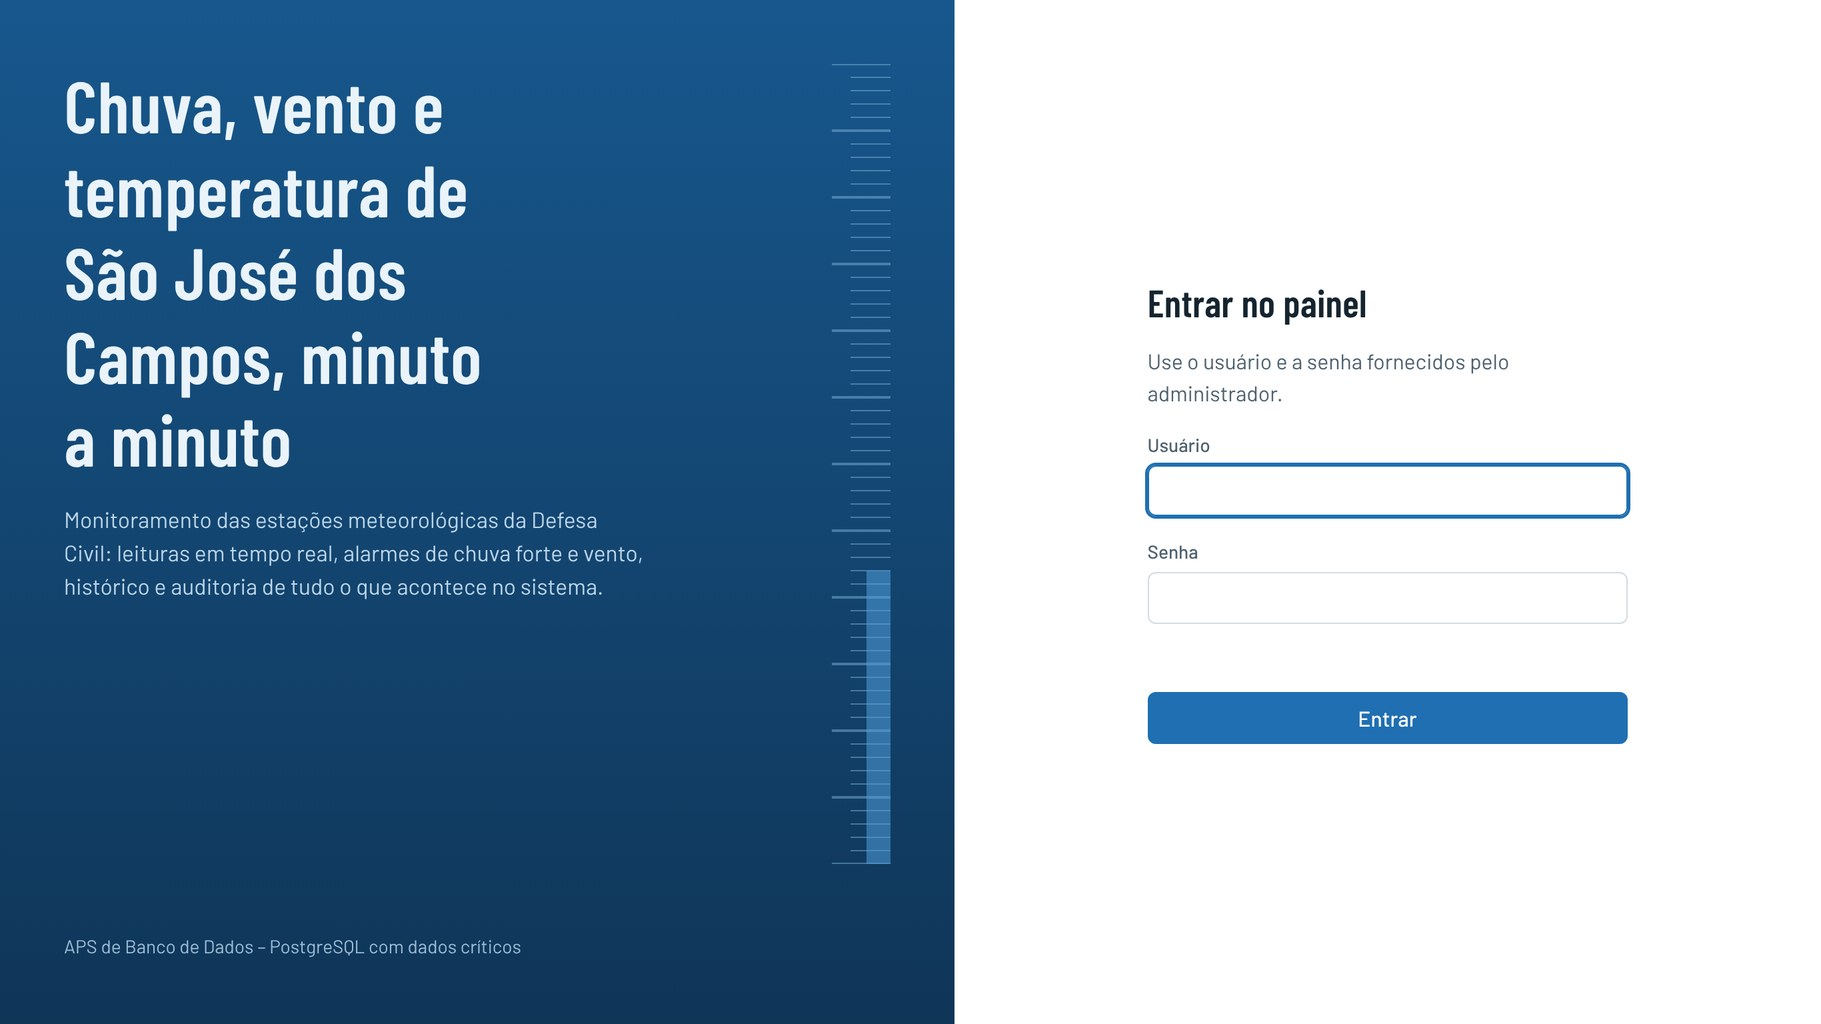
\includegraphics[width=0.80\textwidth]{figuras/login.jpg}
  \fonte{Elaborado pelos autores (2026).}
\end{figure}

O painel (\autoref{fig:painel}) responde em uma frase se as estações estão normais. Cada estação tem um pluviômetro que enche com a chuva do dia até a linha do limite crítico, a temperatura com a tendência das últimas seis horas e as demais grandezas. Os números de hoje e os últimos alarmes e falhas ficam abaixo, e tudo se atualiza sozinho quando chega um lote. O relógio do topo mostra a hora do servidor, não a do computador do usuário.

\begin{figure}[htbp]
  \caption{Painel em tempo real}\label{fig:painel}
  \centering
  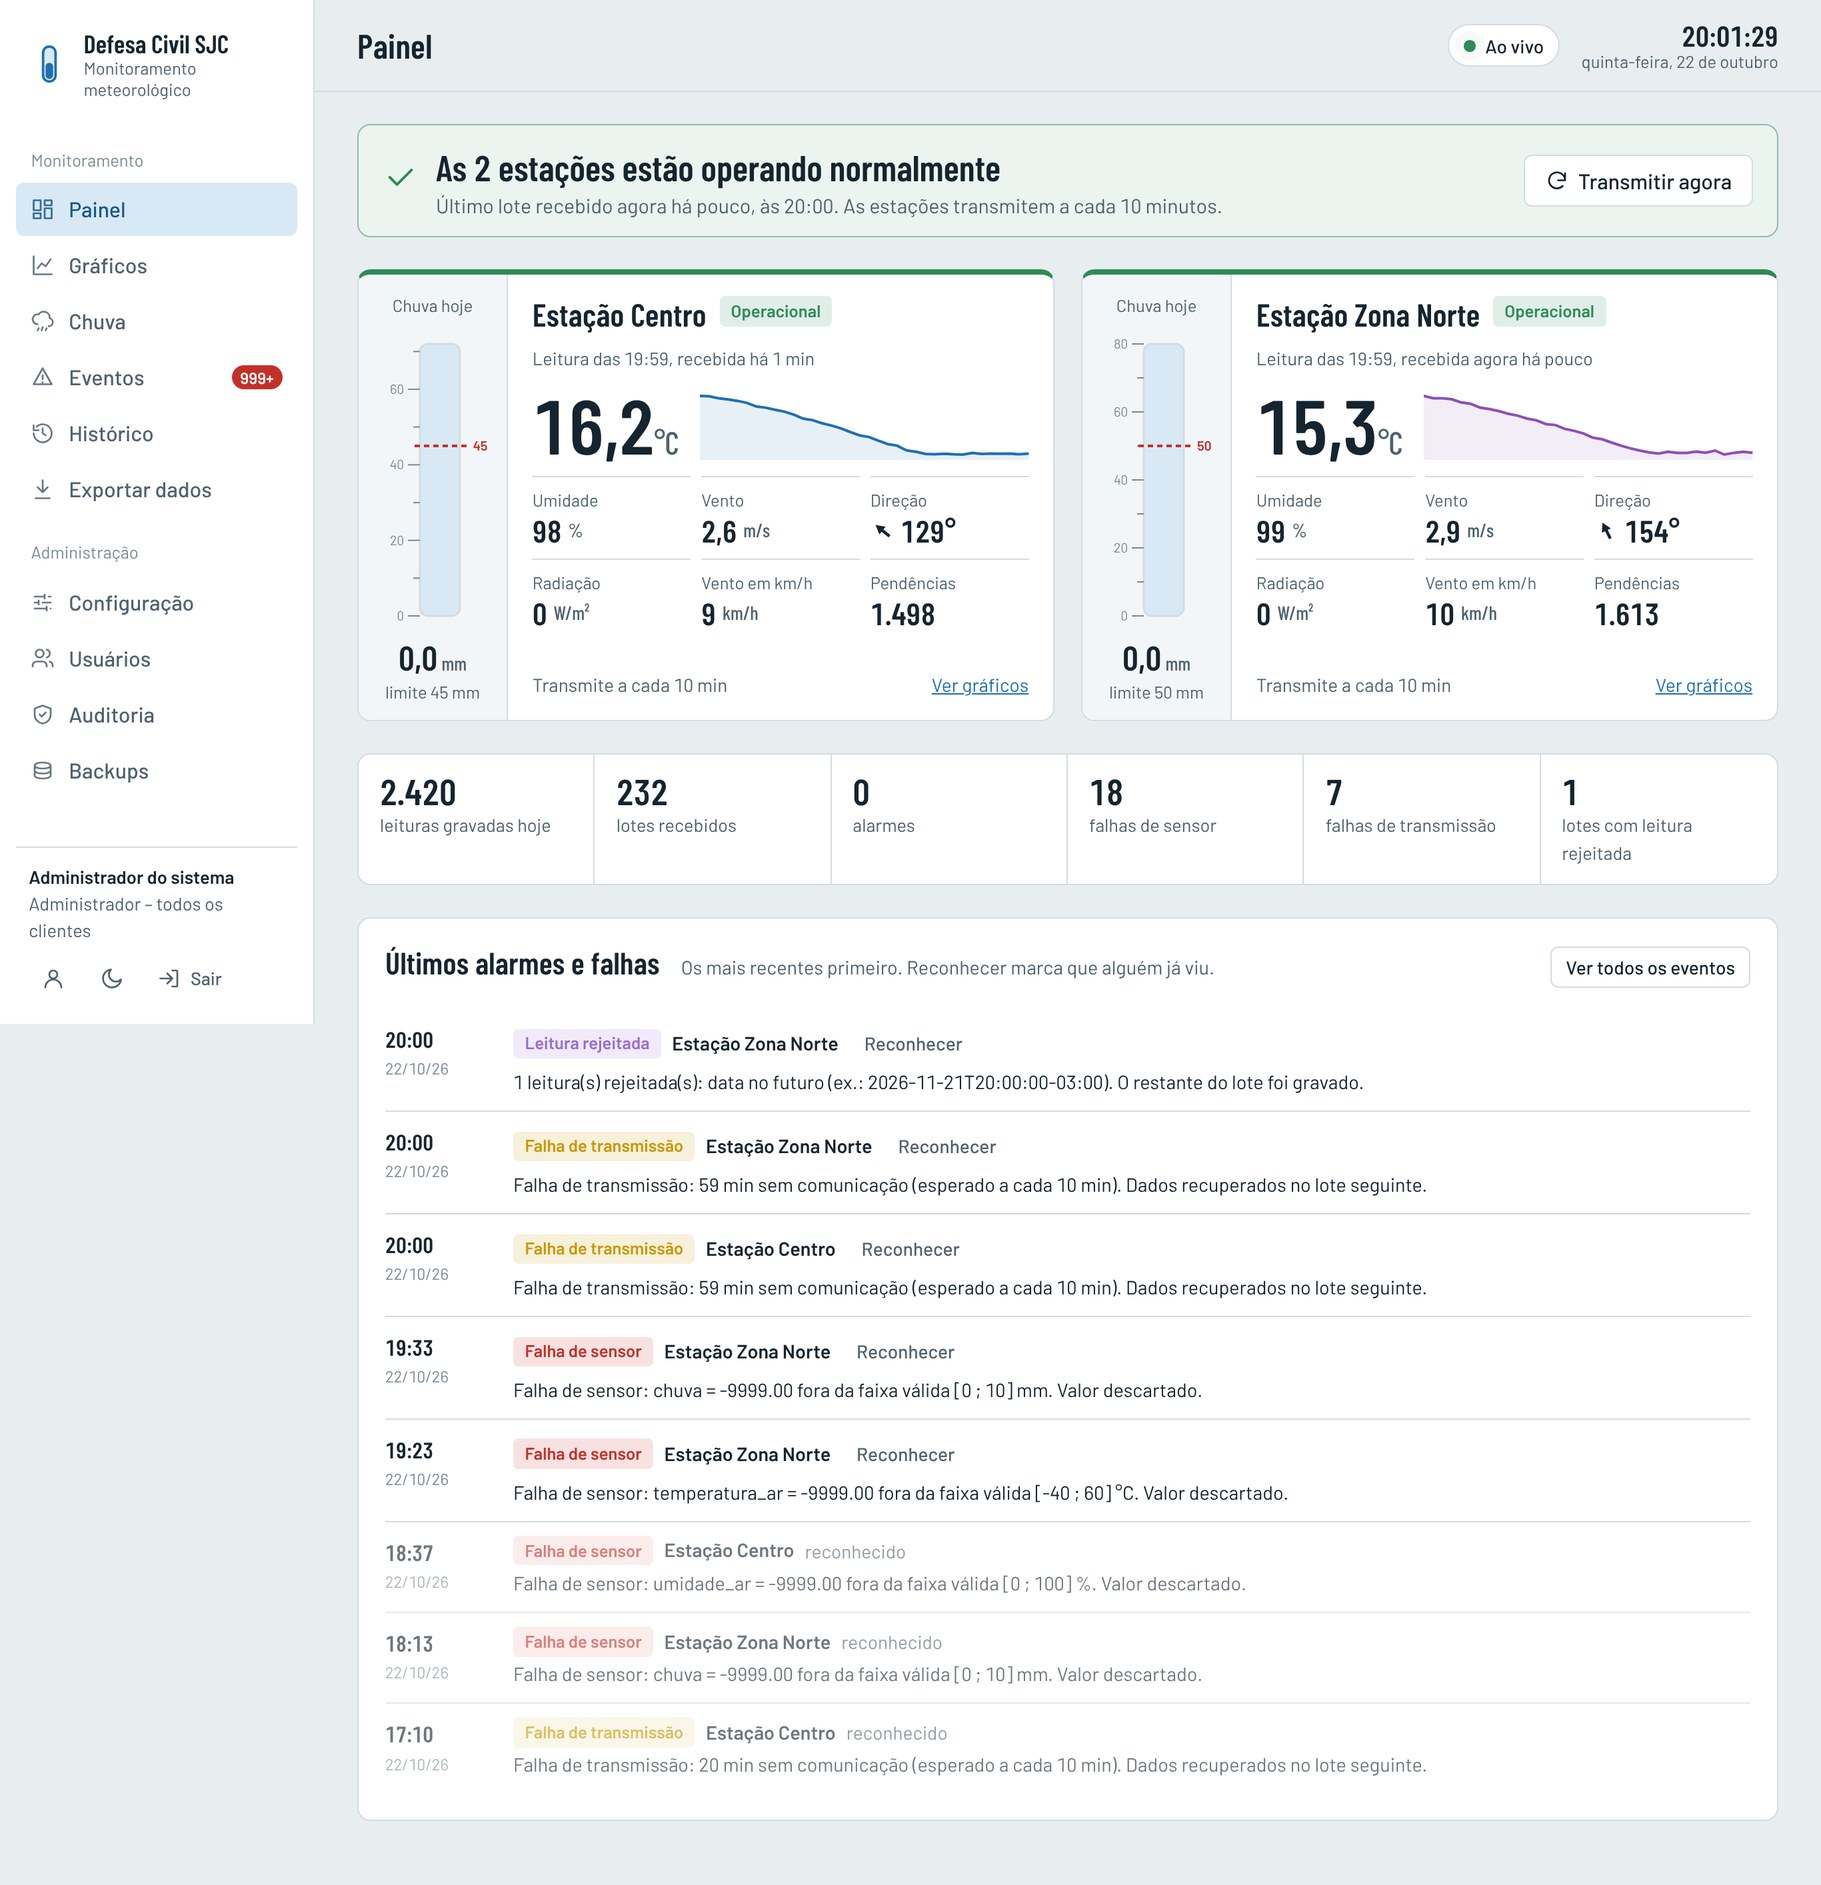
\includegraphics[width=0.68\textwidth]{figuras/painel.jpg}
  \fonte{Elaborado pelos autores (2026).}
\end{figure}

O painel também tem tema escuro, próprio para salas de operação, e se adapta à tela do celular (\autoref{fig:escuro-celular}). No celular, o usuário mostrado é um operador, e o menu não exibe as telas exclusivas do administrador.

\begin{figure}[htbp]
  \caption{Tema escuro e versão para celular}\label{fig:escuro-celular}
  \centering
  \begin{minipage}[c]{0.66\textwidth}
    \centering
    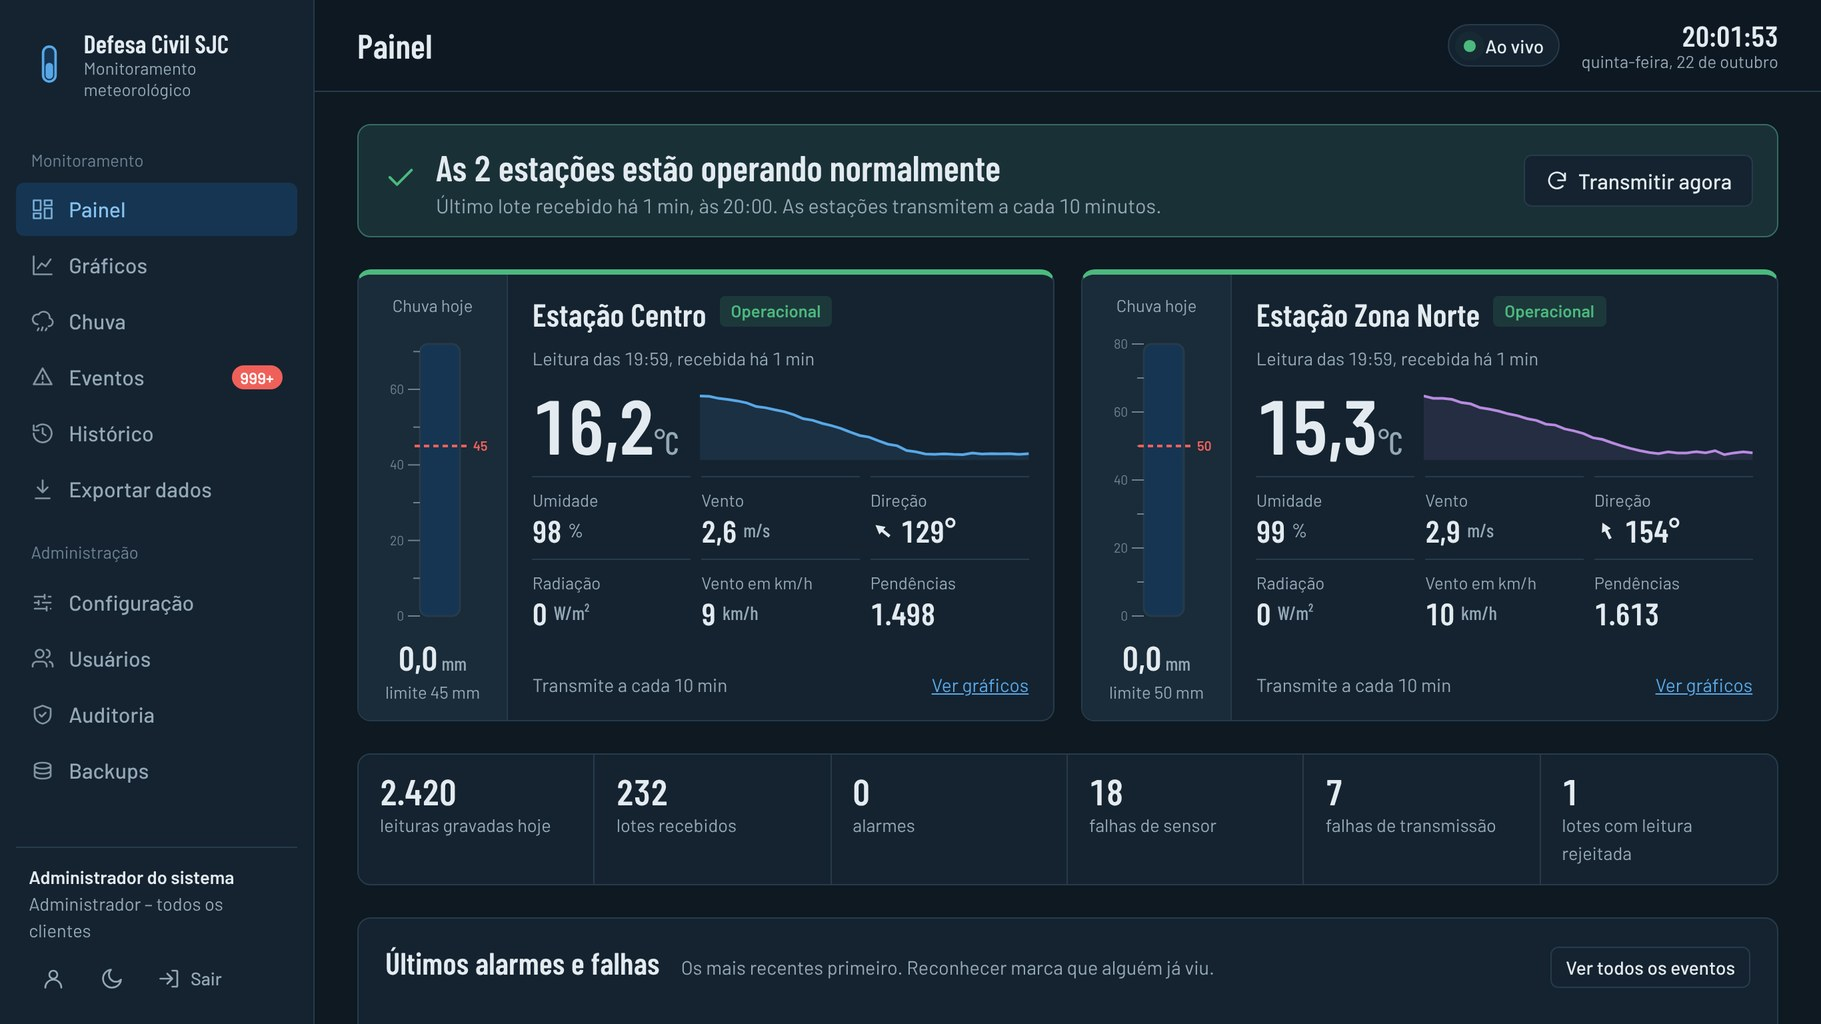
\includegraphics[width=\textwidth]{figuras/painel_escuro.jpg}
  \end{minipage}\hfill
  \begin{minipage}[c]{0.245\textwidth}
    \centering
    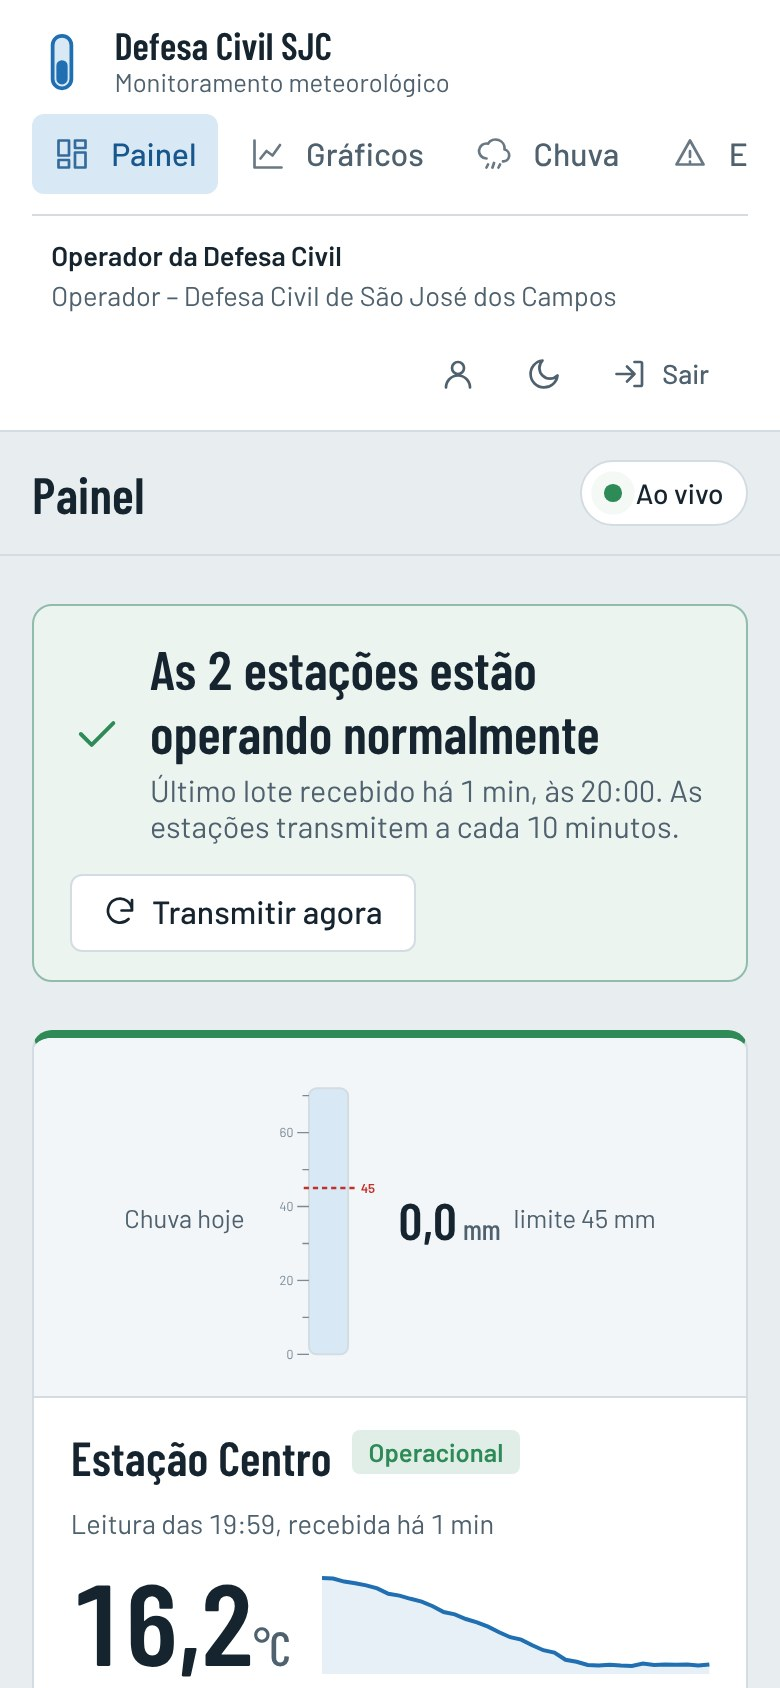
\includegraphics[width=\textwidth]{figuras/celular.jpg}
  \end{minipage}
  \fonte{Elaborado pelos autores (2026).}
\end{figure}

A tela de gráficos (\autoref{fig:graficos}) mostra temperatura, umidade, vento e radiação em 24 horas, 7 ou 30 dias, com as linhas dos limites de alarme. Os gráficos são desenhados em SVG pelo próprio painel, sem bibliotecas externas.

\begin{figure}[htbp]
  \caption{Gráficos com limites de alarme}\label{fig:graficos}
  \centering
  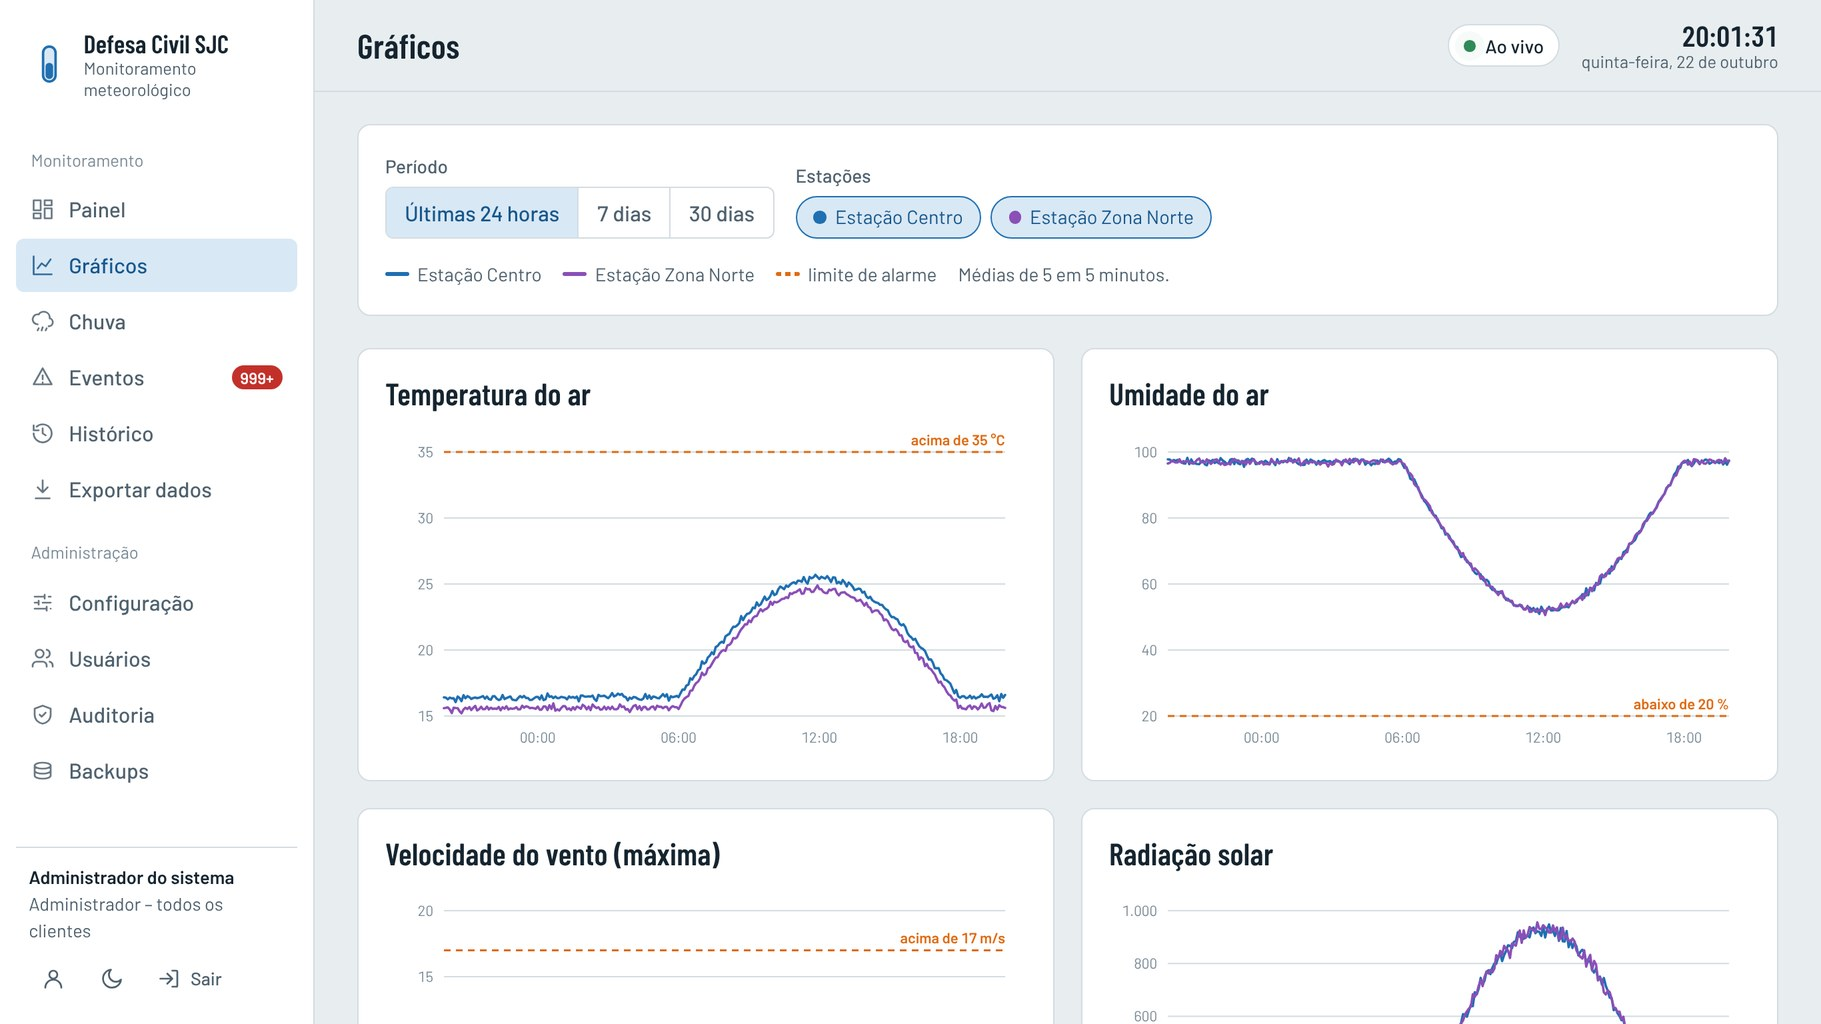
\includegraphics[width=0.80\textwidth]{figuras/graficos.jpg}
  \fonte{Elaborado pelos autores (2026).}
\end{figure}

A tela de eventos (\autoref{fig:eventos}) permite filtrar por tipo, estação e período e reconhecer eventos em lote. Para cada evento reconhecido, mostra quem reconheceu e quando, informações preenchidas pelo banco.

\begin{figure}[htbp]
  \caption{Eventos e reconhecimento}\label{fig:eventos}
  \centering
  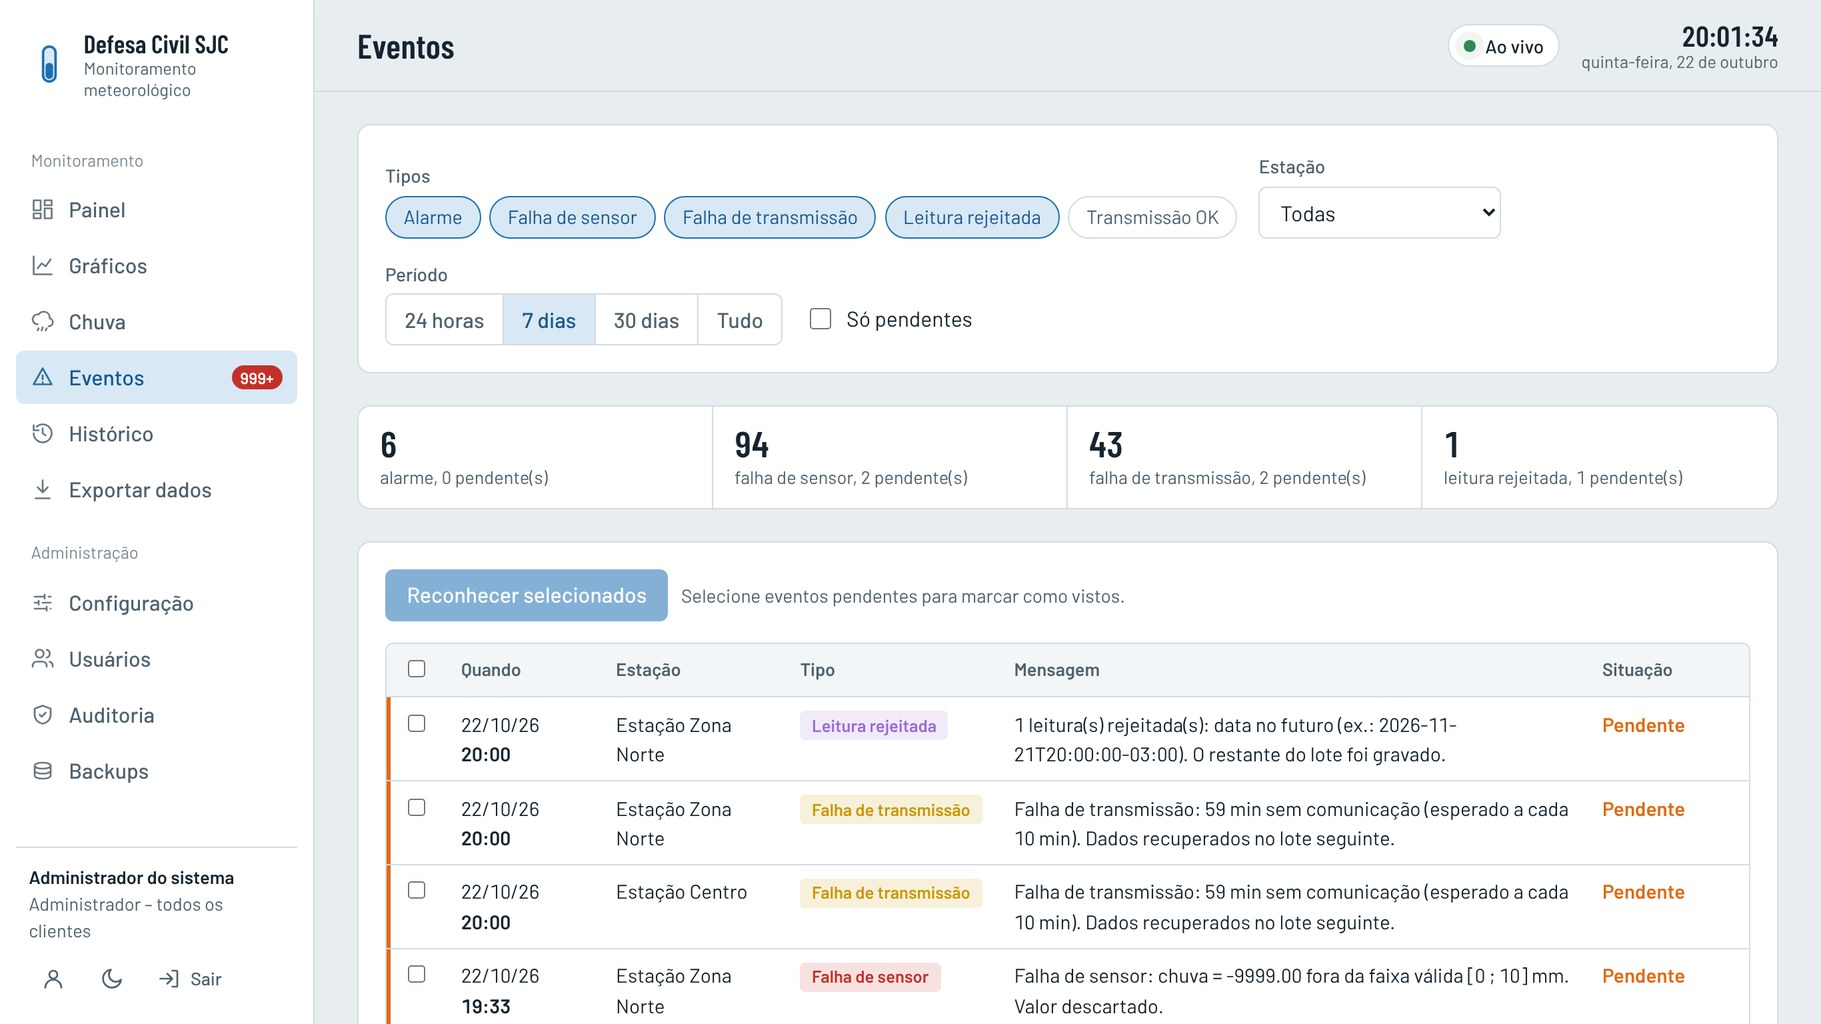
\includegraphics[width=0.80\textwidth]{figuras/eventos.jpg}
  \fonte{Elaborado pelos autores (2026).}
\end{figure}

A tela de configuração (\autoref{fig:config}) permite ao operador ajustar as regras de alarme e as faixas dos sensores; os parâmetros de datas e retenção só podem ser alterados pelo administrador. Cada alteração vai para a auditoria com os valores de antes e depois.

\begin{figure}[htbp]
  \caption{Configuração das regras de alarme}\label{fig:config}
  \centering
  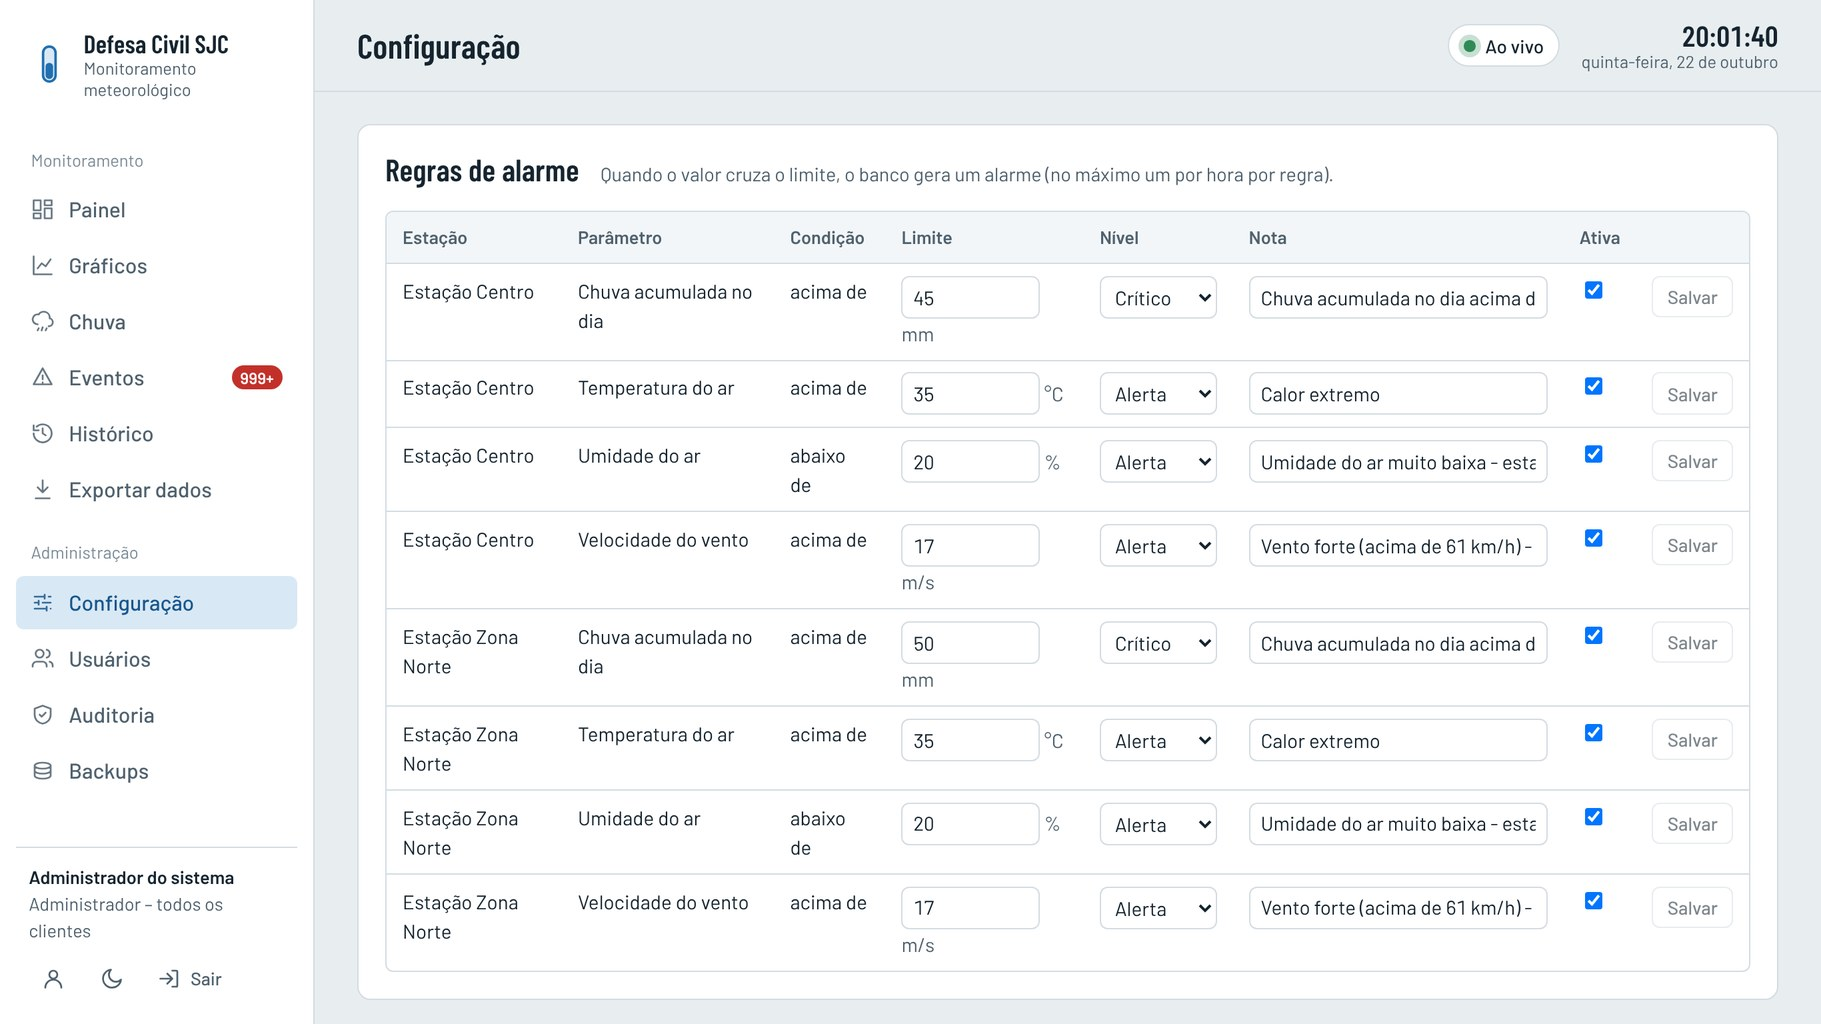
\includegraphics[width=0.80\textwidth]{figuras/config.jpg}
  \fonte{Elaborado pelos autores (2026).}
\end{figure}

Na tela de usuários (\autoref{fig:usuarios}), o administrador cadastra pessoas com perfil e cliente, redefine senhas, desativa e desbloqueia contas. A senha provisória é gerada aleatoriamente e precisa ser trocada no primeiro acesso.

\begin{figure}[htbp]
  \caption{Gestão de usuários}\label{fig:usuarios}
  \centering
  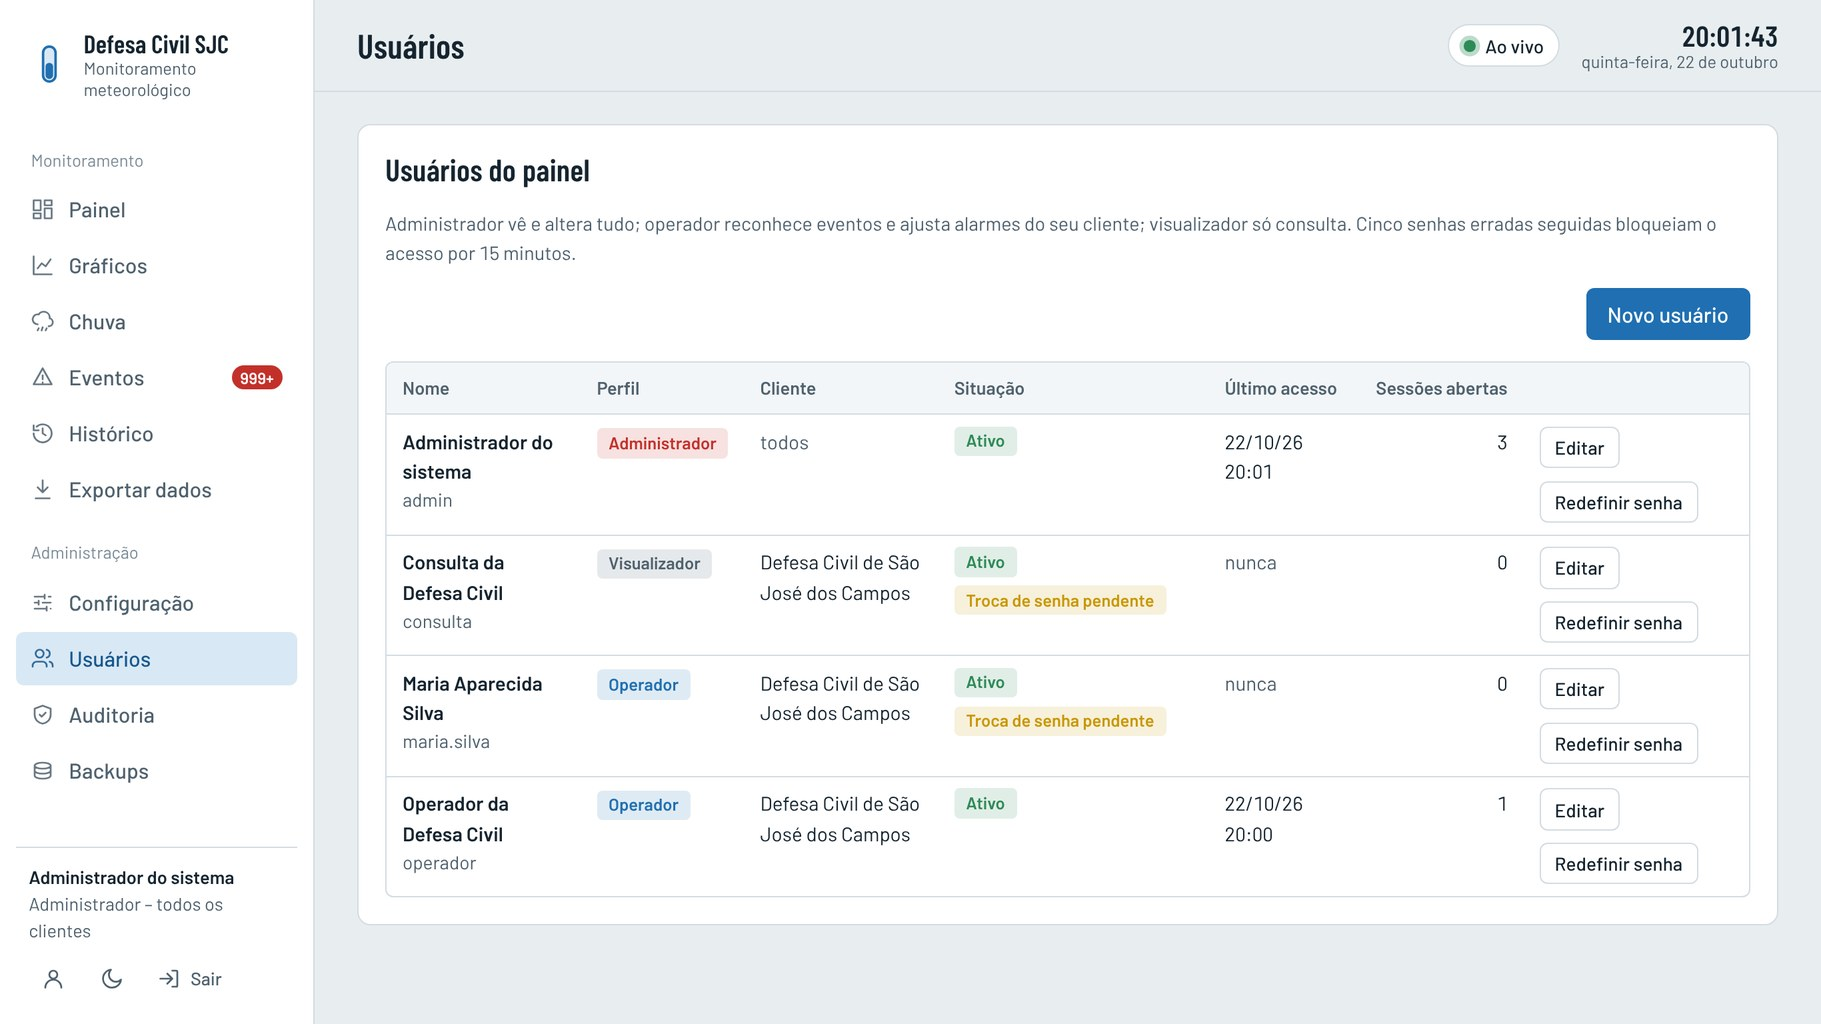
\includegraphics[width=0.80\textwidth]{figuras/usuarios.jpg}
  \fonte{Elaborado pelos autores (2026).}
\end{figure}

A tela de auditoria (\autoref{fig:auditoria}) verifica a corrente de hashes ao abrir e lista cada ação com usuário, IP, objeto e detalhe. Na figura, o registro 49 mostra o operador alterando o limite de chuva da Estação Centro de 50 para 45~mm, e o registro 686, outra alteração da mesma regra, aberta com o antes e depois de cada campo.

\begin{figure}[htbp]
  \caption{Auditoria com antes e depois de uma alteração}\label{fig:auditoria}
  \centering
  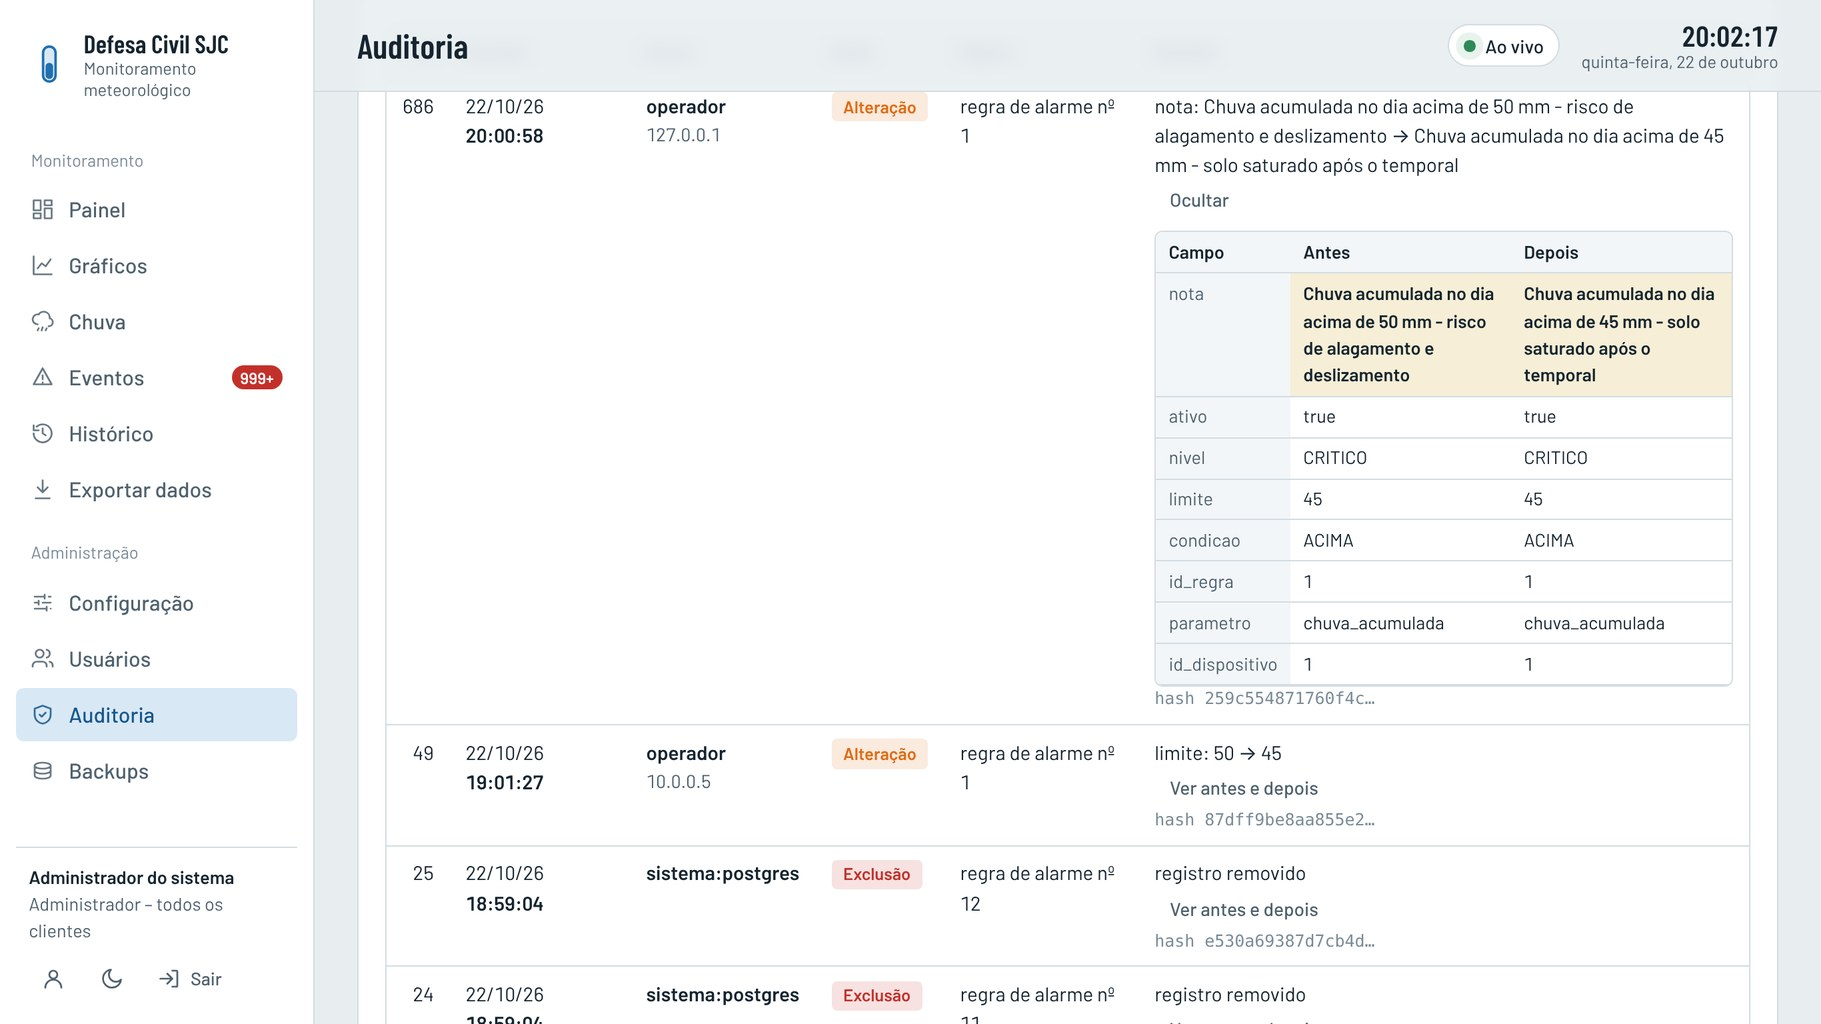
\includegraphics[width=0.80\textwidth]{figuras/auditoria_diff.jpg}
  \fonte{Elaborado pelos autores (2026).}
\end{figure}

A tela de backups (\autoref{fig:backups}) mostra a última cópia, a próxima automática, os parâmetros de durabilidade do PostgreSQL, a fila de contingência e o plano de recuperação. Cada cópia pode ser verificada e baixada; ambas as ações ficam na auditoria.

\begin{figure}[htbp]
  \caption{Backups e continuidade}\label{fig:backups}
  \centering
  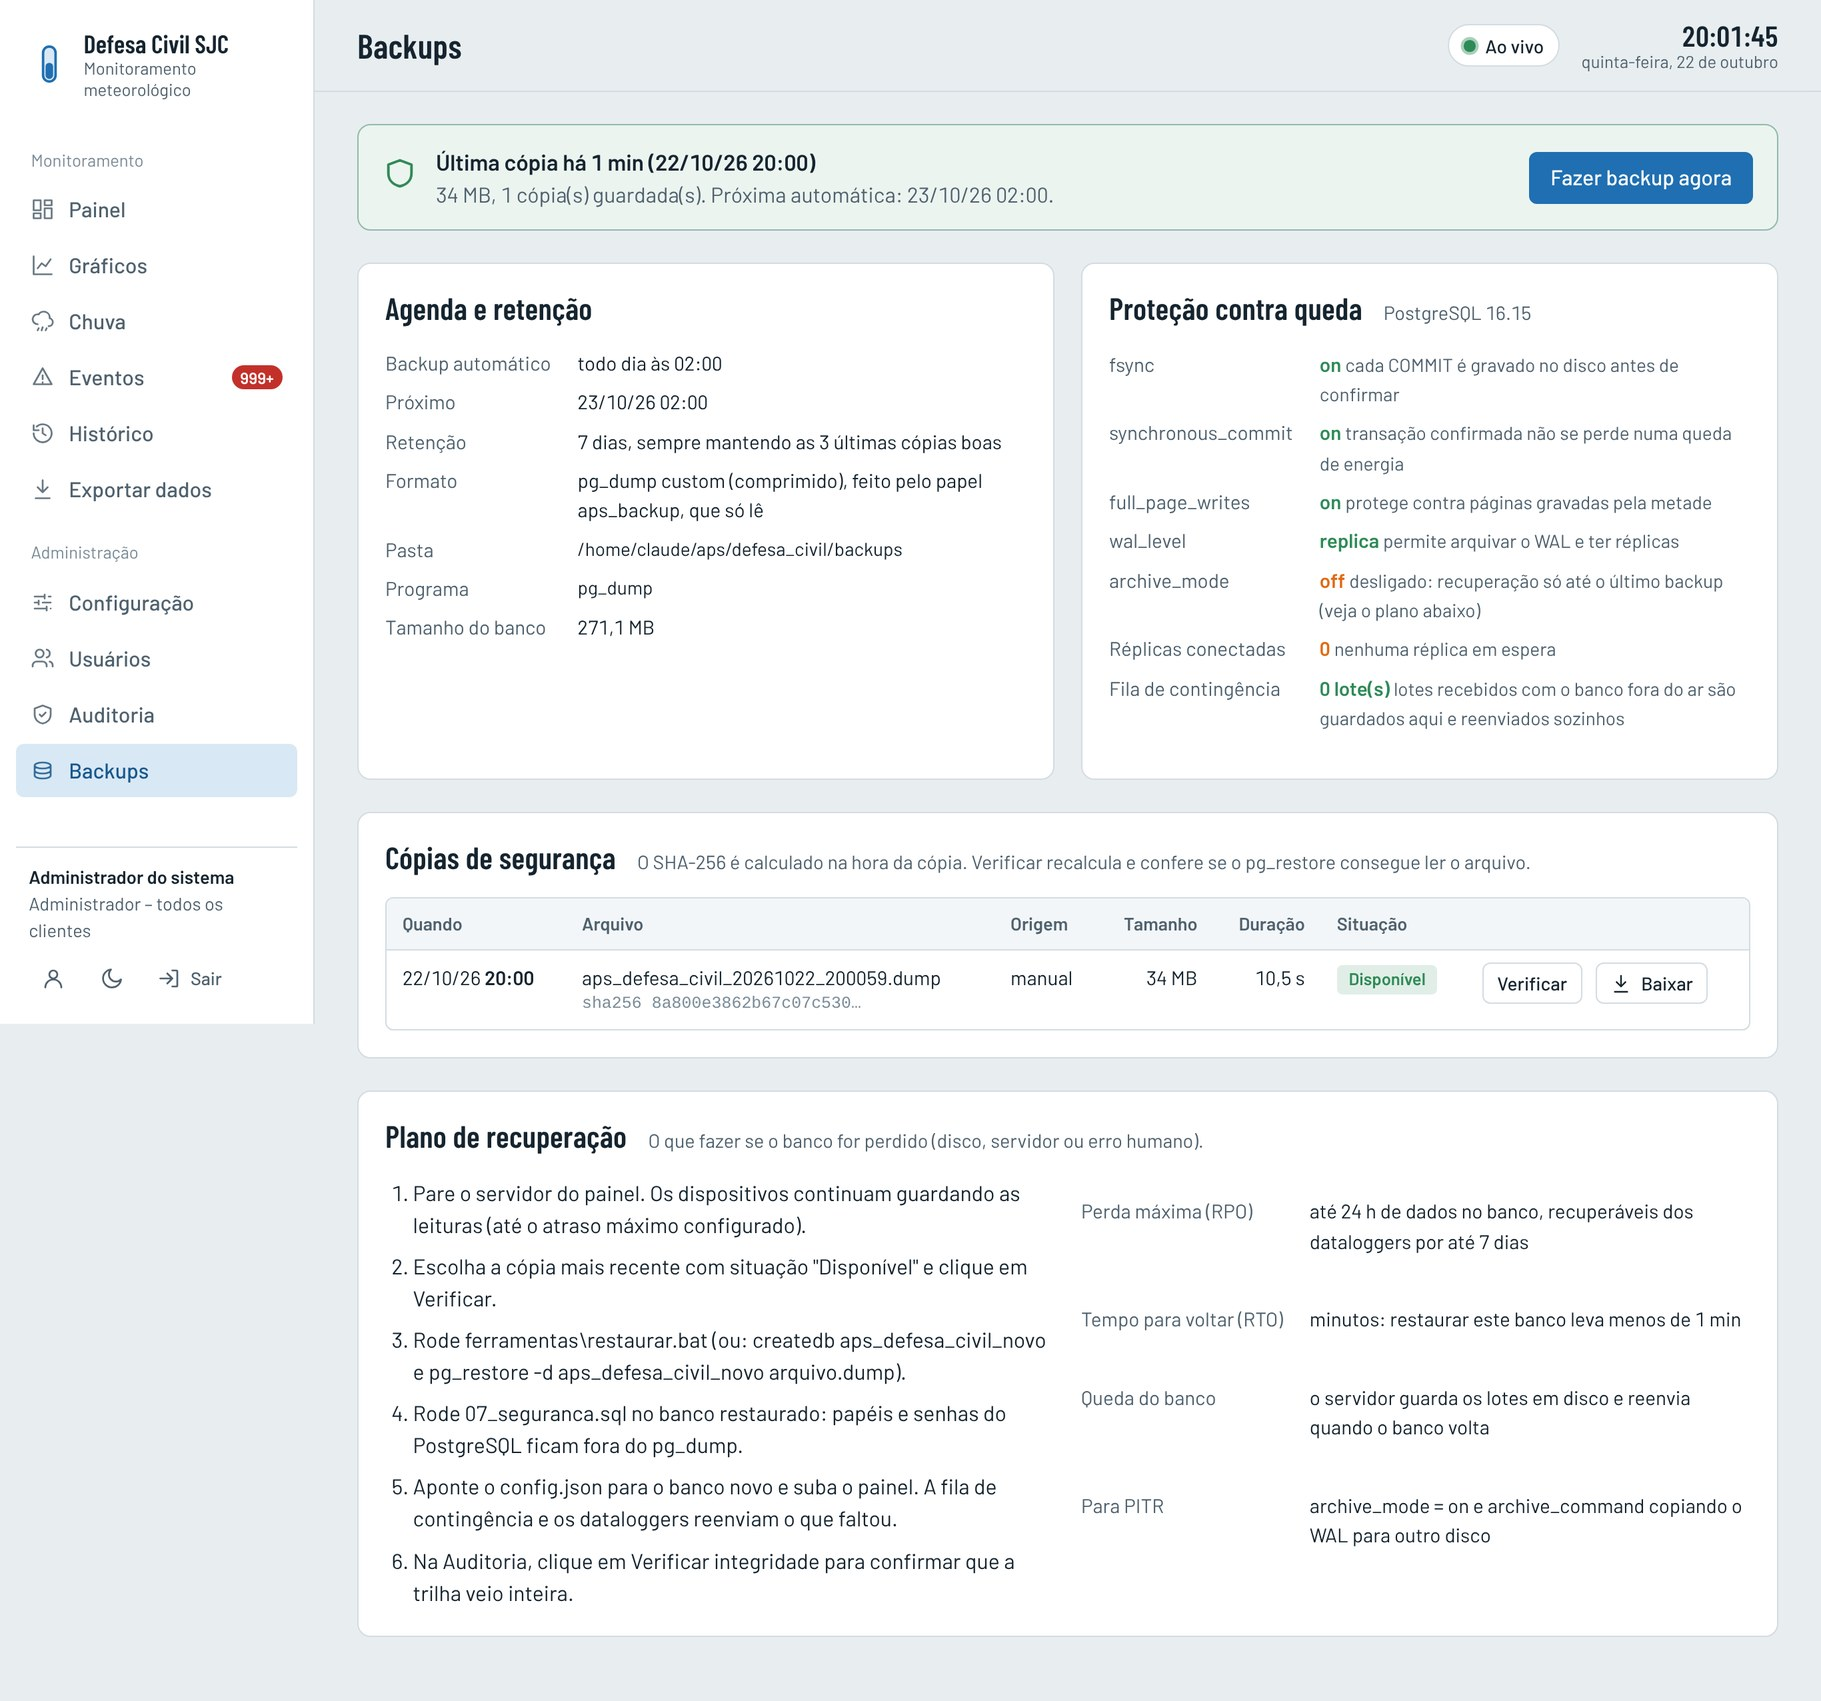
\includegraphics[width=0.68\textwidth]{figuras/backups.jpg}
  \fonte{Elaborado pelos autores (2026).}
\end{figure}

Por fim, a tela de histórico (\autoref{fig:historico}) mostra o ciclo de vida dos dados: os meses arquivados, os ativos e as partições já criadas para os meses seguintes, além do resumo mensal de cada estação.

\begin{figure}[htbp]
  \caption{Histórico e ciclo de vida dos dados}\label{fig:historico}
  \centering
  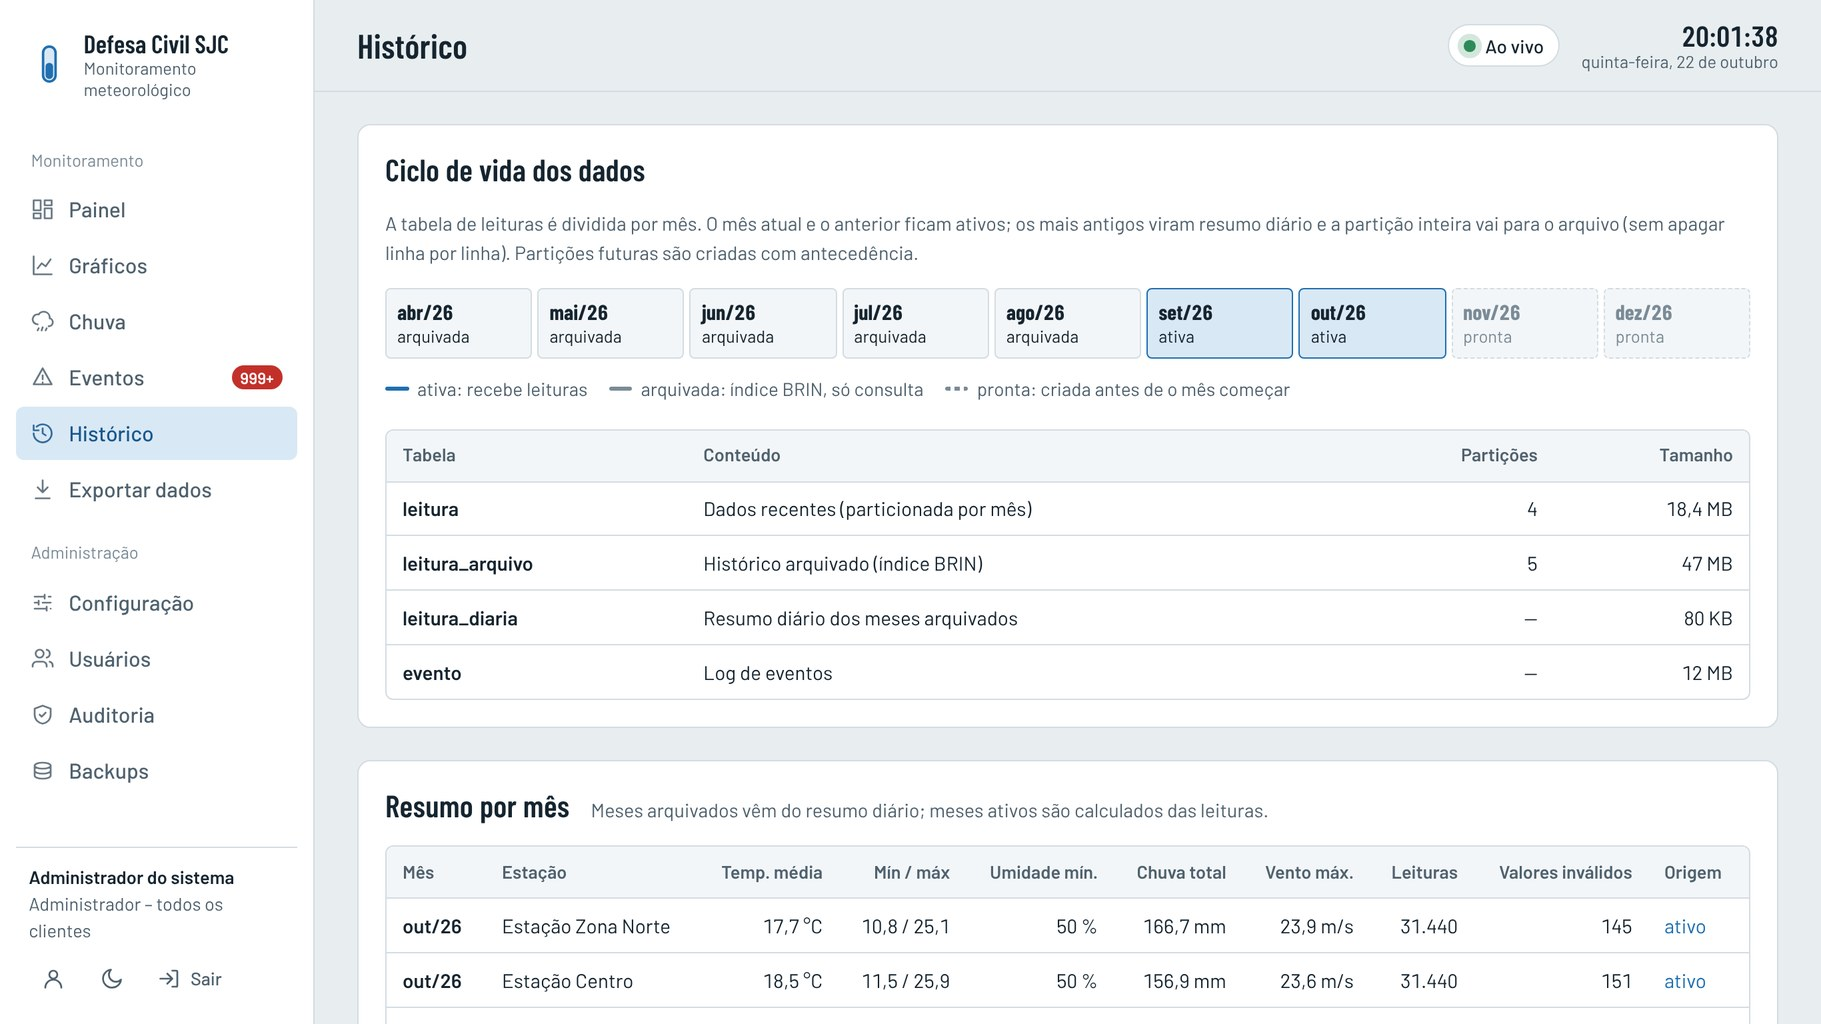
\includegraphics[width=0.80\textwidth]{figuras/historico.jpg}
  \fonte{Elaborado pelos autores (2026).}
\end{figure}

% =====================================================================
\chapter[Por que o protótipo atende a dados críticos]{Por que o protótipo atende a dados \mbox{críticos}}\label{cap:criticos}
% =====================================================================

Um sistema serve a dados críticos quando cada uma das propriedades da \autoref{sec:fund-criticos} (integridade, confidencialidade, disponibilidade e rastreabilidade) é garantida por um mecanismo concreto, e quando esse mecanismo resiste a quem tenta contorná-lo. O \autoref{qua:criticos} relaciona cada ameaça ao mecanismo implementado e ao teste que comprova seu funcionamento; os testes estão detalhados no \autoref{cap:resultados}.

\begin{quadro}[htbp]
  \caption{Garantias de dados críticos no protótipo}\label{qua:criticos}
  \scriptsize
  \begin{tabularx}{\textwidth}{|L{2.0cm}|L{3.4cm}|Y|L{1.3cm}|}
    \hline
    \textbf{Propriedade} & \textbf{Ameaça} & \textbf{Mecanismo} & \textbf{Teste} \\ \hline
    \multirow{4}{2.0cm}{Integridade}
      & Leitura com data errada no relógio do equipamento & Validação por leitura contra o relógio do servidor; rejeição registrada, sem descartar o lote & S08, S07 \\ \cline{2-4}
      & Aplicação grava dado com data escolhida por ela & Função pública sem parâmetro de data; versão com data negada aos papéis da aplicação & S06 \\ \cline{2-4}
      & Valor inválido do sensor ($-9999$) contamina médias & Faixa física por sensor; valor anulado e evento registrado & Carga \\ \cline{2-4}
      & Alteração de evento já registrado & Evento imutável; só o reconhecimento muda, com data e usuário do banco & S10 \\ \hline
    \multirow{3}{2.0cm}{Confidencia\-lidade}
      & Servidor web invadido & Papéis de mínimo privilégio; banco valida o \textit{token} da sessão a cada transação & S01, S02 \\ \cline{2-4}
      & Usuário vê dados de outro cliente & RLS por cliente em todas as tabelas de dados & S01, S03 \\ \cline{2-4}
      & Senha descoberta por força bruta & bcrypt; bloqueio de 15 min após 5 erros; sessão só como hash & S11 \\ \hline
    \multirow{2}{2.0cm}{Rastreabi\-lidade}
      & Limite de alarme elevado sem deixar rastro & Auditoria com antes e depois, usuário, IP e data do servidor & S04 \\ \cline{2-4}
      & Apagar ou alterar a própria auditoria & Trilha somente de inclusão, encadeada por SHA-256; DDL também auditado & S12, S13 \\ \hline
    \multirow{4}{2.0cm}{Disponi\-bilidade}
      & Virada do mês sem partição & Criação automática das partições futuras & S09 \\ \cline{2-4}
      & Banco fora do ar & Fila de contingência em disco com reenvio automático & C1 \\ \cline{2-4}
      & Perda do servidor ou erro humano & Backup diário verificado por SHA-256, retenção e restauração testada & C2, C3 \\ \cline{2-4}
      & Queda de energia & WAL com \texttt{fsync} e \texttt{synchronous\_commit} ligados & Config. \\ \hline
  \end{tabularx}
  \fonte{Elaborado pelos autores (2026).}
\end{quadro}

Quatro decisões de projeto explicam por que essas garantias são confiáveis, e não apenas declaradas.

\textbf{As regras ficam no banco.} Validação, eventos, perfis e auditoria são implementados em PL/pgSQL, com \textit{triggers} e políticas que valem para qualquer cliente do banco: o painel novo, o painel antigo em Streamlit, um script ou uma ferramenta de administração. Isso segue a ideia de que o SGBD deve concentrar as restrições de integridade e de autorização \parencite{elmasri2018}. Os papéis da aplicação nem sequer têm permissão de inclusão direta nas tabelas de leituras e eventos; só podem chamar as funções que aplicam as regras.

\textbf{O banco não confia na aplicação.} Em vez de receber da aplicação o número do usuário, o que permitiria a um servidor comprometido se passar por qualquer pessoa, o banco recebe o \textit{token} da sessão e o valida na tabela de sessões, onde só o hash está guardado. O isolamento por cliente usa o mesmo mecanismo. Assim, o servidor web é tratado como uma camada potencialmente hostil, aplicando o mínimo privilégio de \textcite{saltzer1975} também entre aplicação e banco.

\textbf{O tempo é do servidor.} Toda data de registro (recebimento, reconhecimento, auditoria, sessão, configuração e backup) vem do relógio do servidor, e as datas das leituras, que vêm do equipamento, são conferidas contra ele. Em dados críticos, a ordem e o momento dos fatos fazem parte do dado: saber que o alarme de chuva foi reconhecido às 15h12, e por quem, só tem valor se ninguém puder escrever outra hora.

\textbf{A rastreabilidade é verificável.} Uma trilha de auditoria comum pode ser editada por quem tem acesso ao banco. A trilha encadeada por hash \parencite{schneier1999,haber1991} não impede um superusuário de alterar uma linha, mas torna essa alteração detectável e aponta onde ela ocorreu. O próprio ato de desligar a proteção fica registrado como comando de estrutura. Combinada com a cópia de segurança, que guarda a trilha num momento anterior, essa verificação permite reconstruir o que foi alterado.

Essas medidas também atendem ao que a LGPD exige para os dados pessoais dos usuários (nome, login e endereço IP): controle de acesso, registro das operações e proteção contra acessos não autorizados \parencite{lgpd2018}. As senhas não são guardadas em forma recuperável, e a auditoria nunca registra a senha nem o seu hash, apenas o fato de que ela foi alterada.

% =====================================================================
\chapter{Resultados e discussão}\label{cap:resultados}
% =====================================================================

Os testes foram executados em Linux (Ubuntu 24.04), com PostgreSQL 16.15 e Node.js 22, sempre sobre um banco recriado do zero.

\section{Carga e detecção de eventos}

A carga gerou 529.250 leituras de seis meses, com todas as validações ativas. O arquivamento manteve os dois meses mais recentes na tabela principal (149.090 leituras), moveu os anteriores para o arquivo (380.160) e gerou 264 dias de resumo. Foram registrados, nas estações Centro e Zona Norte, respectivamente, \num{25928} e \num{25955} transmissões OK, 523 e 501 falhas de transmissão, \num{1280} e \num{1358} falhas de sensor e 16 e 17 alarmes, valores próximos das taxas simuladas. No dia de temporal, as duas estações geraram alarme de vento e alarme crítico de chuva, e a chuva acumulada pelo \textit{trigger} coincidiu com a soma das leituras.


\section{Testes de segurança e continuidade}

Os testes de segurança (\autoref{qua:testes-seg}) usaram o papel do servidor web (\texttt{aps\_app}), como faria um invasor que tivesse tomado o servidor, e a API do painel. Todos tiveram o resultado esperado; o S12 mostra que nem o superusuário altera o passado sem ser percebido.

\begin{quadro}[htb]
  \caption{Testes de segurança e integridade}\label{qua:testes-seg}
  \scriptsize
  \begin{tabularx}{\textwidth}{|c|Y|Y|}
    \hline
    \textbf{ID} & \textbf{Tentativa} & \textbf{Resultado} \\ \hline
    S01 & Consultar dados sem sessão & Nenhuma linha visível (RLS) \\ \hline
    S02 & Usar \textit{token} de sessão falso & Nenhuma linha; ações recusadas \\ \hline
    S03 & Operador lê usuários e auditoria & Permissão negada; zero linhas \\ \hline
    S04 & Operador altera limite de alarme (permitido) & Gravado e auditado com antes, depois, usuário e IP \\ \hline
    S05 & Operador altera parâmetro de administrador & Nenhuma linha afetada \\ \hline
    S06 & Aplicação grava leitura direto, apaga evento ou informa data & Permissão negada nas três \\ \hline
    S07 & Superusuário inclui leitura com data no futuro & Recusada pelo \textit{trigger} \\ \hline
    S08 & Lote com seis leituras, cinco com datas inválidas & 1 gravada; 5 rejeitadas em 3 eventos por motivo \\ \hline
    S09 & Virada de mês sem partição & Manutenção cria o mês atual e os dois seguintes \\ \hline
    S10 & Alterar evento ou desfazer reconhecimento & Recusado: evento imutável \\ \hline
    S11 & Senha errada repetidas vezes & Bloqueio de 15 min na 5ª tentativa \\ \hline
    S12 & Superusuário desliga a proteção e altera a auditoria & Verificação aponta o registro exato; o desligamento fica registrado \\ \hline
    S13 & Apagar registro da auditoria & Recusado: somente inclusão \\ \hline
    S14 & Requisição sem o cabeçalho do painel (CSRF) & Recusada (HTTP 403) \\ \hline
    S15 & Reenviar lote já gravado com $-9999$ & Nenhum evento novo (antes, falha de sensor) \\ \hline
  \end{tabularx}
  \fonte{Elaborado pelos autores (2026).}
\end{quadro}

\begin{quadro}[htb]
  \caption{Testes de continuidade}\label{qua:testes-cont}
  \scriptsize
  \begin{tabularx}{\textwidth}{|c|Y|Y|}
    \hline
    \textbf{ID} & \textbf{Cenário} & \textbf{Resultado} \\ \hline
    C1 & Banco desligado durante envios & Lotes aceitos (HTTP 202) na fila e reenviados em segundos ao religar; painel avisou a queda \\ \hline
    C2 & Backup sob demanda e verificação & 35,6~MB em 10,5~s; SHA-256 conferido; 450 objetos legíveis \\ \hline
    C3 & Restauração em banco novo & Mesmas contagens (149.162, 380.160 e 55.547) e auditoria íntegra \\ \hline
    C4 & Servidor parado por uma hora & Leituras recuperadas; falha de transmissão de 59 min registrada \\ \hline
  \end{tabularx}
  \fonte{Elaborado pelos autores (2026).}
\end{quadro}

Com backup diário, a perda máxima no banco (RPO) é de 24 horas, mas na prática é menor, pois as estações guardam as leituras e o banco aceita reenvios de até sete dias; a restauração (RTO) leva minutos. O arquivamento contínuo do WAL reduziria o RPO a minutos \parencite{pgbackup}.

\section{Desempenho e custo das validações}

Na escrita de 1.000 pontos (média de 20 repetições), comparando a primeira versão e a final, o envio de um ponto por vez passou de 946,8 para 1.245,8~ms ($+31{,}6\,\%$), e o envio em lotes de dez, de 226,9 para 235,3~ms ($+3{,}7\,\%$). As validações são feitas uma vez por lote, por isso o custo se dilui no envio em lotes, modo de operação das estações, 5,3 vezes mais rápido que o unitário, como observado por \textcite{grzesik2020}.


\begin{figure}[htb]
  \caption{Tempo médio das consultas por cenário (500 repetições, escala logarítmica)}\label{fig:consultas}
  \centering
  \begin{tikzpicture}
    \begin{axis}[
      width=0.92\textwidth, height=4.8cm,
      ybar, bar width=9pt, area legend, ymode=log, log origin=infty,
      ymin=0.08, ymax=150,
      symbolic x coords={Q1,Q2,Q3,Q4},
      xtick=data, enlarge x limits=0.18,
      ylabel={tempo médio (ms)},
      ylabel style={font=\footnotesize}, tick label style={font=\footnotesize},
      log ticks with fixed point, yticklabel style={/pgf/number format/use comma},
      legend style={font=\scriptsize, at={(0.5,1.03)}, anchor=south, legend columns=4, draw=none},
      ymajorgrids, grid style={cinza!25},
      axis line style={cinza},
    ]
      \addplot[fill=cinza!70, draw=none]   coordinates {(Q1,28.82) (Q2,31.34) (Q3,32.76) (Q4,63.31)};
      \addplot[fill=azul!55, draw=none]    coordinates {(Q1,0.45) (Q2,34.41) (Q3,33.42) (Q4,11.00)};
      \addplot[fill=verde!70, draw=none]   coordinates {(Q1,0.38) (Q2,6.54) (Q3,7.91) (Q4,11.10)};
      \addplot[fill=azul, draw=none]       coordinates {(Q2,0.16) (Q3,0.18)};
      \legend{A sem índice, B índice composto, C particionada, D view materializada}
    \end{axis}
  \end{tikzpicture}
  \fonte{Elaborada pelos autores (2026). Q1: uma estação em 1 dia; Q2 e Q3: médias, mínimos e máximos de 7 dias; Q4: vento por dia em 30 dias.}
\end{figure}

Nas consultas (\autoref{fig:consultas}), o índice composto foi o melhor para uma estação (Q1, 64 vezes mais rápida), a view materializada foi de 185 a 200 vezes mais rápida nas agregações de vários dias (Q2 e Q3) e o particionamento reduziu o tempo de 4 a 6 vezes. Ler a chuva acumulada foi 4,3 vezes mais rápido que somar as leituras do dia. No PostgreSQL 18, o índice composto também acelerou Q2 e Q3 de 5 a 6,6 vezes, graças ao \textit{skip scan} \parencite{pg18release}.

% =====================================================================
\chapter{Conclusão}\label{cap:conclusao}
% =====================================================================

O trabalho atingiu o objetivo de projetar e prototipar um banco de dados de telemetria IoT adequado a dados críticos. A primeira versão já recebia leituras em volume e gerava alarmes, mas não protegia o dado contra perda, adulteração e acesso indevido; as melhorias fecharam essas lacunas e foram comprovadas por testes.

Três conclusões se destacam. Primeiro, \textbf{as garantias de um dado crítico devem ficar no banco}: validação, imutabilidade, perfis, isolamento por cliente e auditoria valem para qualquer programa, e o servidor web tratado como invadido não leu nada sem um \textit{token} válido. Segundo, \textbf{rastreabilidade só vale se for verificável}: a auditoria encadeada por hash apontou o registro exato alterado pelo próprio superusuário. Terceiro, \textbf{segurança tem custo mensurável e controlável}: menos de 4\,\% no envio em lotes, com as consultas mantendo ganhos de até 200 vezes.

Para a Defesa Civil, cada leitura chega validada e com data confiável, uma estação que para de transmitir é identificada, uma chuva acima do limite gera alarme no mesmo minuto, e nada se perde se o banco cair por algumas horas. As principais limitações são os dados simulados e de pequeno volume, o formato largo, que exige alterar a tabela para um novo tipo de sensor, e os testes em um único computador. Como trabalhos futuros, ficam: ativar o arquivamento do WAL e uma réplica; publicar o último hash da auditoria fora do servidor; usar HTTPS e autenticação em dois fatores; conectar uma estação real; e enviar alertas automáticos à população e às equipes.


% =====================================================================
% ELEMENTOS PÓS-TEXTUAIS
% =====================================================================
\postextual
\printbibliography[title=Referências]



\end{document}
